%! TeX program = lualatex
\documentclass[a4paper,11pt]{article} 
% packages
\usepackage{censor}
\StopCensoring
\usepackage{fontspec}
\setmainfont{EB Garamond}
% for tironian et fallback
% % \directlua{luaotfload.add_fallback
% % ("emojifallback",
% %      {"Noto Serif:mode=harf"}
% % )}
% % \setmainfont{EB Garamond}[RawFeature={fallback=emojifallback}]

\setmonofont[Scale=MatchLowercase]{Deja Vu Sans Mono}
\usepackage[a4paper,left=2cm,right=2cm,top=\dimexpr15mm+1.5\baselineskip,bottom=2cm]{geometry}
\setlength{\parindent}{0pt}

\usepackage{fancyhdr}       % Headers and footers 
\fancyhead[R]{\normalfont \leftmark}
\fancyhead[L]{}
\pagestyle{fancy}

\usepackage{microtype}      % Slightly tweak font spacing for aesthetics
\usepackage[english]{babel} % Language hyphenation and typographical rules
\usepackage{xcolor}
\definecolor{linkblue}{RGB}{0, 64, 128}
\usepackage[final, colorlinks = false, urlcolor = linkblue]{hyperref} 
% \newcommand{\secref}[1]{\textbf{§~\nameref{#1}}}
\newcommand{\secref}[1]{\textbf{§\ref{#1}~\nameref{#1}}}
\usepackage{array}
\usepackage{amsmath}

\usepackage{changepage}     % adjust margins on the fly


\usepackage{minted}
\usemintedstyle{algol_nu}

\usepackage{pgfplots}
\pgfplotsset{width=\textwidth,compat=1.9}

\usepackage{caption}
\newenvironment{code}{\captionsetup{type=listing}}{}
\captionsetup[listing]{skip=0pt}
\setlength{\abovecaptionskip}{5pt}
\setlength{\belowcaptionskip}{5pt}

\usepackage[yyyymmdd]{datetime}
\renewcommand{\dateseparator}{--}

\usepackage{enumitem}

\usepackage{titlesec}

\author{Andrew Hayes}

\begin{document}
\begin{titlepage}
    \begin{center}
        \hrule
        \vspace*{0.6cm}
        \huge \textbf{CT417}
        \vspace*{0.6cm}
        \hrule
        \LARGE
        \vspace{0.5cm}
            Software Engineering III
        \vspace{0.5cm}
        \hrule

        \vfill
        \vfill

        \hrule
        \begin{minipage}{0.495\textwidth} 
            \vspace{0.4em}
            \raggedright
            \normalsize 
            Name: Andrew Hayes \\
            E-mail: \href{mailto://a.hayes18@universityofgalway.ie}{\texttt{a.hayes18@universityofgalway.ie}}  \hfill\\
            Student ID: 21321503 \hfill
        \end{minipage}
        \begin{minipage}{0.495\textwidth} 
            \raggedleft
            \vspace*{0.8cm}
            \Large
            \today
            \vspace*{0.6cm}
        \end{minipage}
        \medskip\hrule 
    \end{center}
\end{titlepage}

\pagenumbering{roman}
\newpage
\tableofcontents
\newpage
\setcounter{page}{1}
\pagenumbering{arabic}

\section{Introduction}
\subsection{Lecturer Contact Details}
\begin{itemize}
    \item   Dr. Effirul Ramlan.
    \item   Email: \href{mailto://effirul.ramlan@universityofgalway.ie}{\texttt{effirul.ramlan@universityofgalway.ie}}.
    \item   Will attempt to reply to emails immediately between the hours of 09:00 \& 20:00 from Week 01 to
            Week 12.
    \item   Discord server: \url{https://discord.gg/CRAtHv9uNg}.
\end{itemize}

\subsection{Grading}
\begin{itemize}
    \item   Continuous Assessment: 40\%.
            \begin{itemize}
                \item   You will work in pairs on a software project with three key submissions across the 12 weeks.
                        Each deliverable will align with the topics covered in the course up to that point, allowing 
                        for continuous progress assessment.
                \item   AS-01: Set up musicFinder and configure the CI/CD pipeline (Week 4).
                \item   AS-02: Testing, Security, \& Expanded Application (Week 8).
                \item   AS-03: Refactoring \& Application Deployment.
            \end{itemize}

    \item   Final Exam: 60\%.
            \begin{itemize}
                \item   Typical 2-hour exam paper covering materials from Week 1 to Week 12, with nothing out of the ordinary --
                        ``You can be sure of that''.
                    \item   ``There is a question on Agile on your final'' -- key differences between agile \& DevOps table.
            \end{itemize}
\end{itemize}

\section{Revision}
\subsection{What is Software?}
\textbf{Software} consists of:
\begin{enumerate}[label=\roman*.]
    \item   Instruction (computer programs) that when executed provide desired features, function, \& performance.
    \item   Data structures (Arrays, Objects, Lists, Dictionaries, Maps, etc.) that enable programs to manipulate information.
    \item   Descriptive information in both hard copy \& virtual format describing the operation \& use.
\end{enumerate}

\subsection{Functional vs Non-Functional Requirements}
\begin{table}[h!]
    \centering

    \begin{tabular}{|>{\arraybackslash}p{0.5\textwidth}|>{\arraybackslash}p{0.5\textwidth}|}
        \hline
        \textbf{Functional Requirement}                                             & \textbf{Non-Functional Requirement} \\
        \hline
        Describes the actions with which the user's work is concerned               & Describes the experience of the user while doing the work \\
        \hline
        A feature or function that can be captured in use-cases                     & A global constraint (and therefore difficult to capture in use-cases) \\
        \hline
        A behaviour that can be analysed via sequence diagrams or state machines    & A software quality \\
        \hline
        can be usually traced back to a single module / class / function            & Usually cannot be implemented in a single module or even program \\
        \hline
    \end{tabular}
    \caption{Functional vs Non-Functional Requirements}
\end{table}

Typical non-functional requirements include: availability, maintainability, performance, privacy, reliablility, scalability, \& security.

\subsection{What is Software Engineering?}
\textbf{Software Engineering} is the field of computer science that deals with the building of software systems that are so large or so complex
that they are built by a team or teams of engineers.
Software Engineering encompasses a process, a collection of methods, \& an array of tools that allow professionals to build high-quality software.
\\\\
\textbf{DevOps} outlines a software development process that increases the delivery of higher quality software by integrating the efforts of the development 
\& IT operation teams.
$$
    \text{DevOps} = \text{Software Engineering} + \text{IT Operations}
$$

\subsection{What are Software Development Life Cycles?}
\textbf{Software Development Life Cycles (SDLC)} refers to a process used by software engineers to design, develop, \& test software.
Each approach focuses on a different aspect of development, from planning to continuous improvement.

\subsection{What is a Framework?}
A \textbf{software framework} is an abstraction in which common code providing generic functionality can be selectively 
overridden or specialised by user providing specific functionality.
\\\\
\textbf{Low-code} is a method of designing \& developing applications using an intuitive GUI \& embedded functionality that reduce 
traditional professional code writing requirements.
\textbf{No-code} is similar to low-code, but for non-technical business users as it allows them to develop software / applications without
having to write a single line of code.

\subsection{Agile \& DevOps}
\subsubsection{What is Agile?}
\textbf{Agile} is a method of software development consisting of:
\begin{itemize}
    \item   \textbf{Iterative \& Incremental Development:} Software is developed in small, workable increments.
    \item   \textbf{Customer-Centric:} Constant feedback from customers to refine requirements.
    \item   \textbf{Frequent Delivery:} Rapid releases of smaller, functional product versions.
    \item   \textbf{Adaptability:} Agile responds to change quickly
\end{itemize}

\subsubsection{Agile Principles}
\begin{itemize}
    \item   \textbf{Individuals \& Interactions:} over processes \& tools.
    \item   \textbf{Working Software:} over comprehensive documentation.
    \item   \textbf{Customer Collaboration:} over contract negotiation.
    \item   \textbf{Responding to Change:} over following a plan.
    \item   \textbf{Quote:} ``The highest priority is to satisfy the customer through early \& continuous delivery of valuable software.''
\end{itemize}

\subsubsection{Agile Frameworks}
Agile methodologies \& frameworks include:
\begin{itemize}
    \item   \textbf{Scrum:} Divides work into sprints (2-4 weeks) with regular stand-ups \& reviews.
    \item   \textbf{Kanban:} Focuses on visualising workflow \& limiting Work-In-Progress (WIP).
    \item   \textbf{XP (eXtreme Programming):} Emphasises technical excellence \& frequent releases.
    \item   \textbf{Lean Development:} Focuses on minimising waste \& maximising value.
\end{itemize}

\subsubsection{What is DevOps?}
\textbf{DevOps} is a culture \& set of practices that integrated development (Dev) \& operations (Ops).
It involves collaboration \& automation between developers \& IT operations for faster delivery of high-quality software.
It also involves continuous integration/continuous delivery (CI/CD) to automate code testing \& deployment.

$$
    \text{DevOps} = \text{Development} + \text{Operations}
$$

\subsubsection{DevOps Core Practices}
DevOps core practices include:
\begin{itemize}
    \item   \textbf{CI/CD Pipelines:} Automating the building, testing, \& deployment of code.
    \item   \textbf{Infrastructure as Code (IaC):} Managing infrastructure through code (e.g., Terraform, Ansible).
    \item   \textbf{Monitoring \& Logging:} Ensures system reliability through real-time tracking \& analysis.
    \item   \textbf{Collaboration \& Communication:} Cross-functional teams sharing ownership of development \& operations tasks.
\end{itemize}

\subsubsection{Key Differences between Agile \& DevOps}
\begin{table}[h!]
    \centering

    \begin{tabular}{|>{\arraybackslash}p{0.5\textwidth}|>{\arraybackslash}p{0.5\textwidth}|}
        \hline
        \textbf{Agile}                                                              & \textbf{DevOps} \\
        \hline
        Focus on frequent customer feedback                                         & Focus on collaboration between Dev \& Ops teams \\
        \hline
        Iteration done through iterative cycles                                     & Iteration done through rapid feedback loops \\
        \hline
        Scope of smaller, incremental changes                                       & Scope of large-scale projects \\
        \hline
        Uses task management software (e.g. Jira)                                   & Uses automation tools (e.g. Jenkins) \\
        \hline
        Scrum, XP frameworks                                                        & Kanban, DevOps lifecycle frameworks \\
        \hline
    \end{tabular}
    \caption{Key Differences between Agile \& DevOps}
\end{table}

\textbf{Agile} focuses on iterative development \& customer feedback, with a short feedback loop.
\textbf{DevOps} focuses on automating delivery, collaboration, \& integration between Dev \& Ops teams, integrating the entire process for faster releases.

\subsubsection{Why DevOps Complements Agile}
Agile improvements development velocity, but DevOps extends the concept to deployment \& maintenance.
Both are customer-focused, but DevOps ensures rapid \& reliable deployment in addition to development.
DevOps fills gaps Agile doesn't cover, like operations, infrastructure, \& automation.
Agile helps development teams iterate \& adapt to changing requirements, while DevOps bridges the gap between developers \& IT operations.

\subsubsection{Benefits of Agile \& DevOps}
\begin{itemize}
    \item   Faster, more frequent delivery of features.
    \item   Improved communication \& collaboration between teams. 
    \item   Reduced risk of deployment errors.
    \item   Ability to adapt to customer feedback \& market changes rapidly.
    \item   Higher-quality software \& reduced time-to-market.
\end{itemize}
 
\section{Version Control}
\subsection{What is Version Control?}
\textbf{Version Control} is a system that records changes to a file or set of files over time, allowing you to recall or access specific versions
at a later date.
It is also known as \textit{revision control} or \textit{source control}.
It allows you to keep track of changes, by whom, \& when they occurred.
Some of the popular version control programs include Git, CVS, Subversion, Team Foundation Server, \& Mercurial.
\\\\
It allows us to:
\begin{itemize}
    \item   Backup the source code and be able to rollback to a previous version.
    \item   Keep a record of who did what and when (know who to praise \& who to fire).
    \item   Collaborate with the team (know who to praise \& who to fire).
    \item   Troubleshoot issues by analysing the change history to figure out what caused the problem.
    \item   Analyse statistics such as who is being the most productive etc.
\end{itemize}

\subsection{What files should be checked in to Version Control?}
Any file that influences the software build should be checked into version control.
This includes configuration files, file encodings, binary settings, etc.
Furthermore, anything that is needed to setup the project from a clean checkout / fork should also be included in the version 
control, such as source code, documentation, manuals, image files, datasets, etc.
\\\\
You should not check in any binary files such as JAR files or any other ``build'' files, any intermediate files from build / 
compilation such as \verb|.pyc| or \verb|.o| files, any files which contain an absolute path, or personal preference /
personal settings files.

\subsection{Centralised Version Control -- Subversion}
\begin{figure}[H]
    \centering
    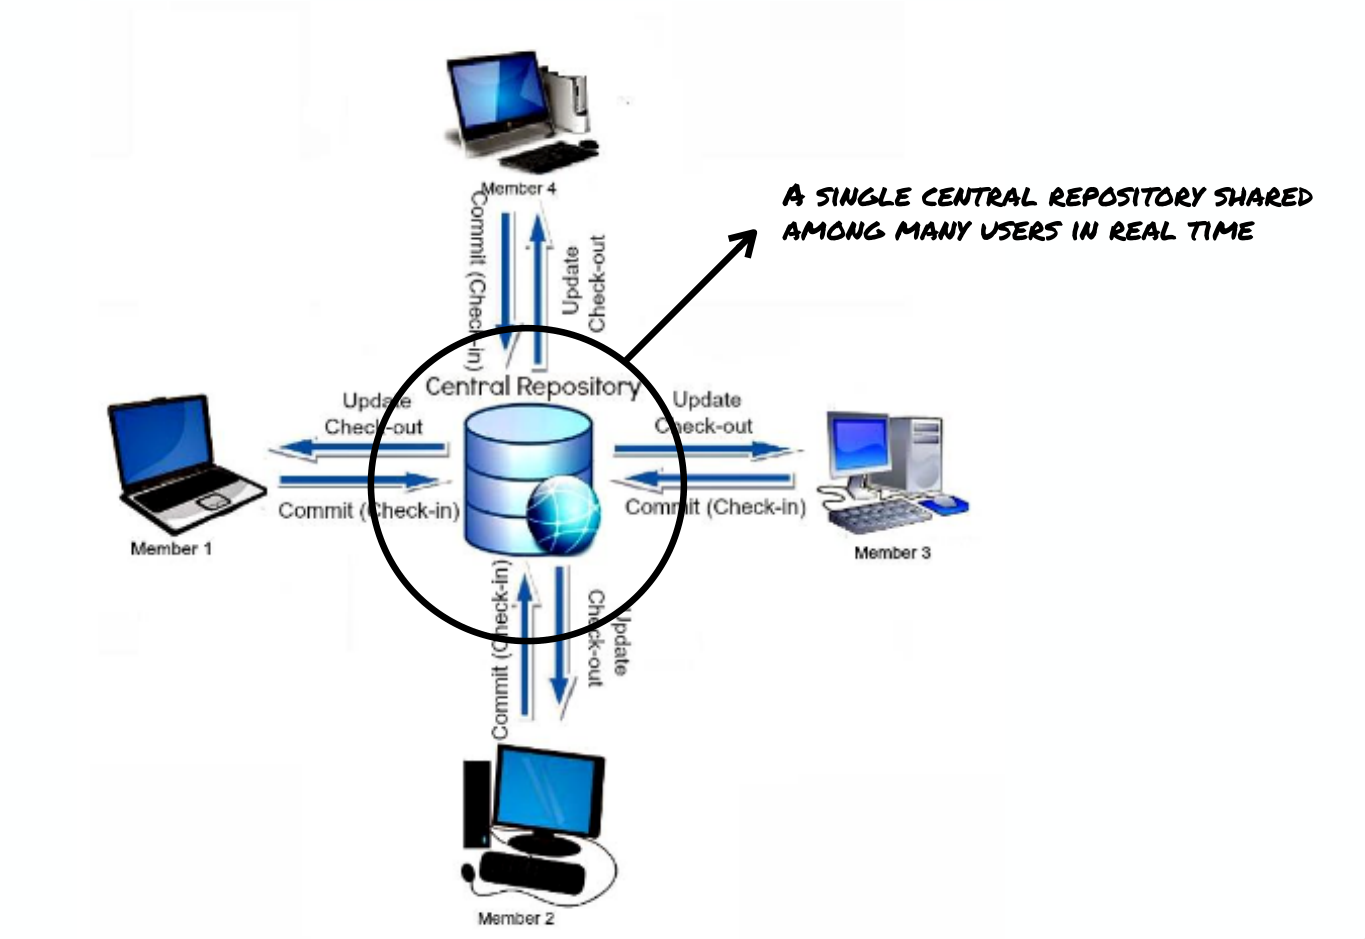
\includegraphics[width=0.8\textwidth]{images/centralised_vcs.png}
    \caption{Centralised Version Control System Diagram}
\end{figure}

\textbf{Subversion} is a centralised version control system in which code is centralised in a repository which can be checked out 
to get a working copy on your local machine.
In general, you don't have the entire repository checked out in Subversion, just a specific branch.
Changes are committed back to the central repository, ``normally'' with useful comments, and a change log is maintained 
of who did what \& when.

\begin{figure}[H]
    \centering
    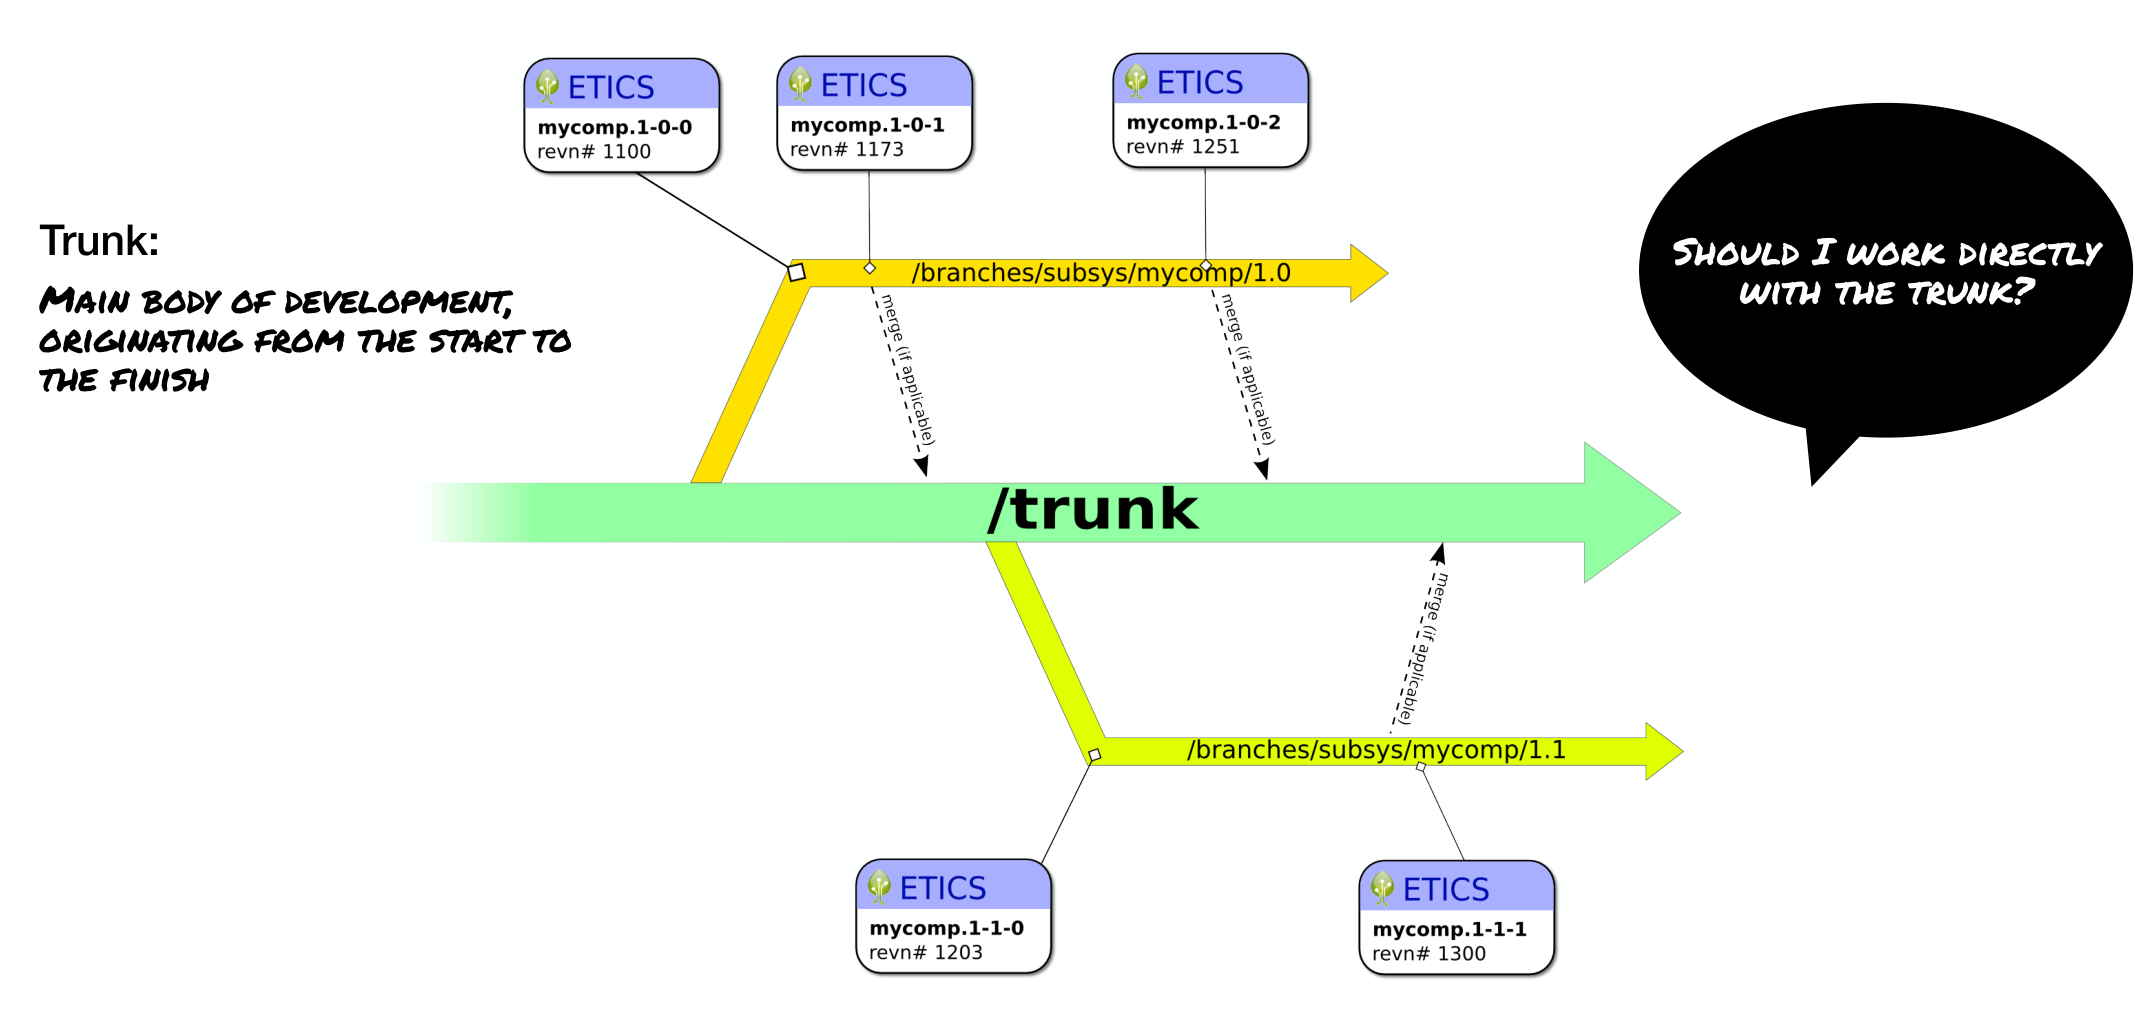
\includegraphics[width=\textwidth]{images/svn_trunk.png}
    \caption{Trunk in Subversion}
\end{figure}

\begin{figure}[H]
    \centering
    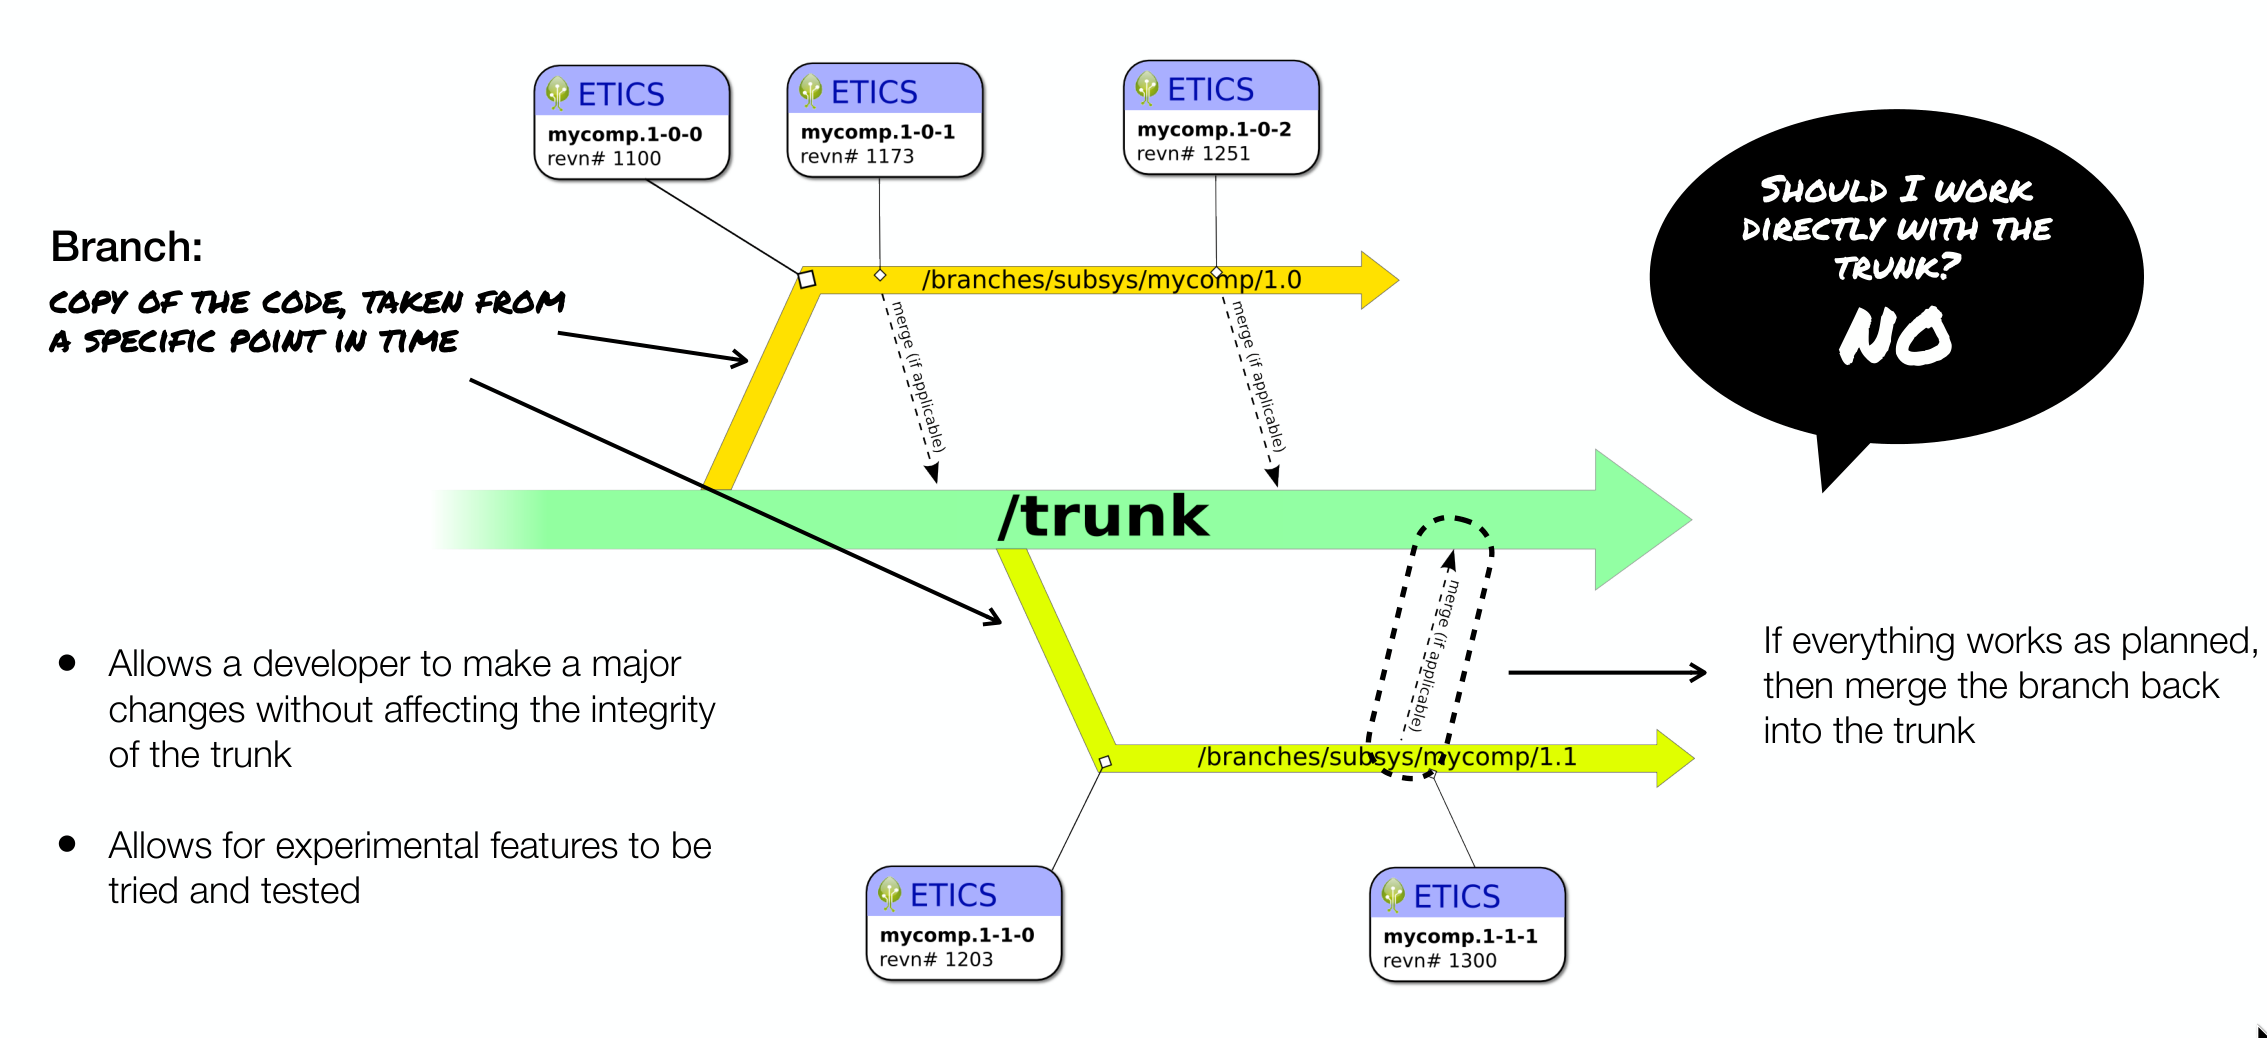
\includegraphics[width=\textwidth]{images/svn_branch.png}
    \caption{Branching in Subversion}
\end{figure}

When you check out the project in subversion, you will get the \verb|HEAD| revision.
When you invoke the command \mintinline{shell}{svn update}, you are updating your local copy to the \verb|HEAD| version
as well.
Branches should eventually be merged back into the trunk with \mintinline{shell}{svn commit}.
The trunk must build afterwards.
The commit is a process of storing changes from your private workplace to the central server.
After the commit, your changes are made available to the rest of the team;
other developers can retrieve these changes by updating their working copy.
Committing is an \textbf{atomic operation}: either the whole commit succeeds, or it is entirely rolled back -- users never
see a half-finished commit.

\begin{figure}[H]
    \centering
    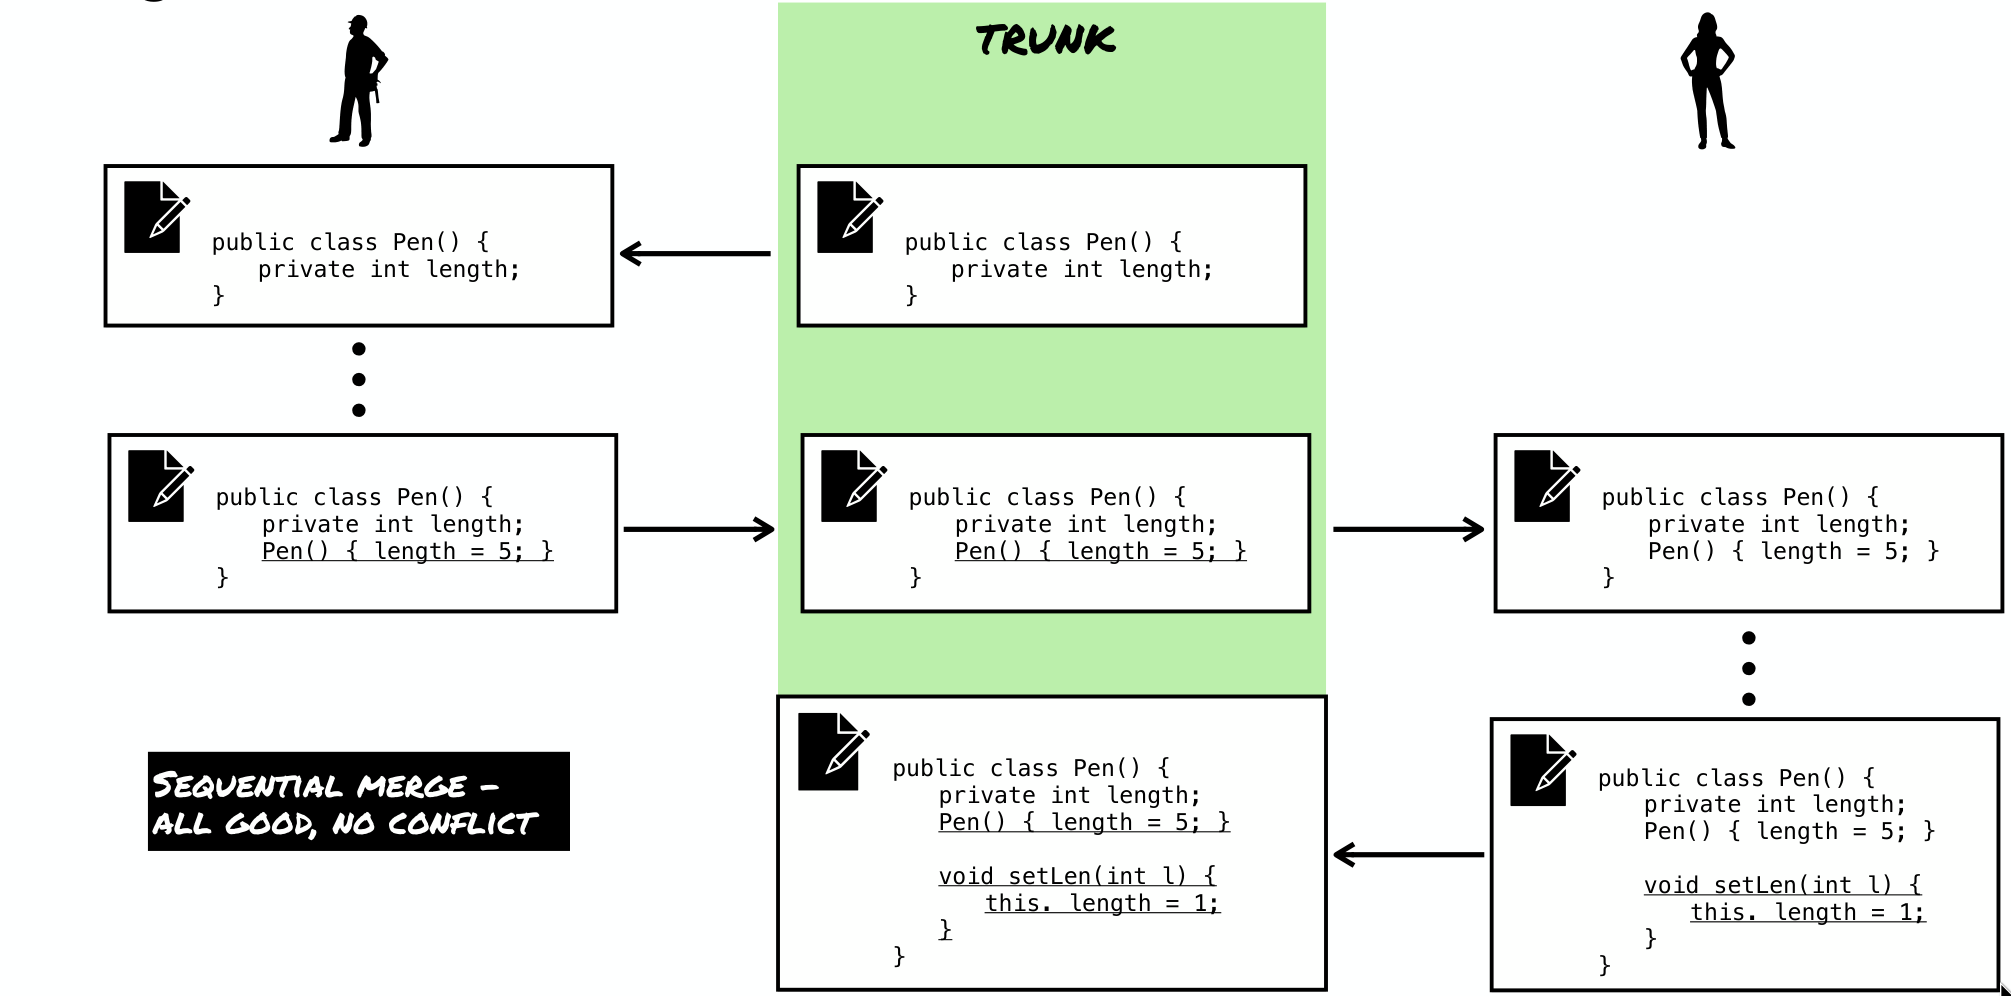
\includegraphics[width=0.8\textwidth]{images/svn_sequential_merge.png}
    \caption{Sequential Merge in Subversion}
\end{figure}

\begin{figure}[H]
    \centering
    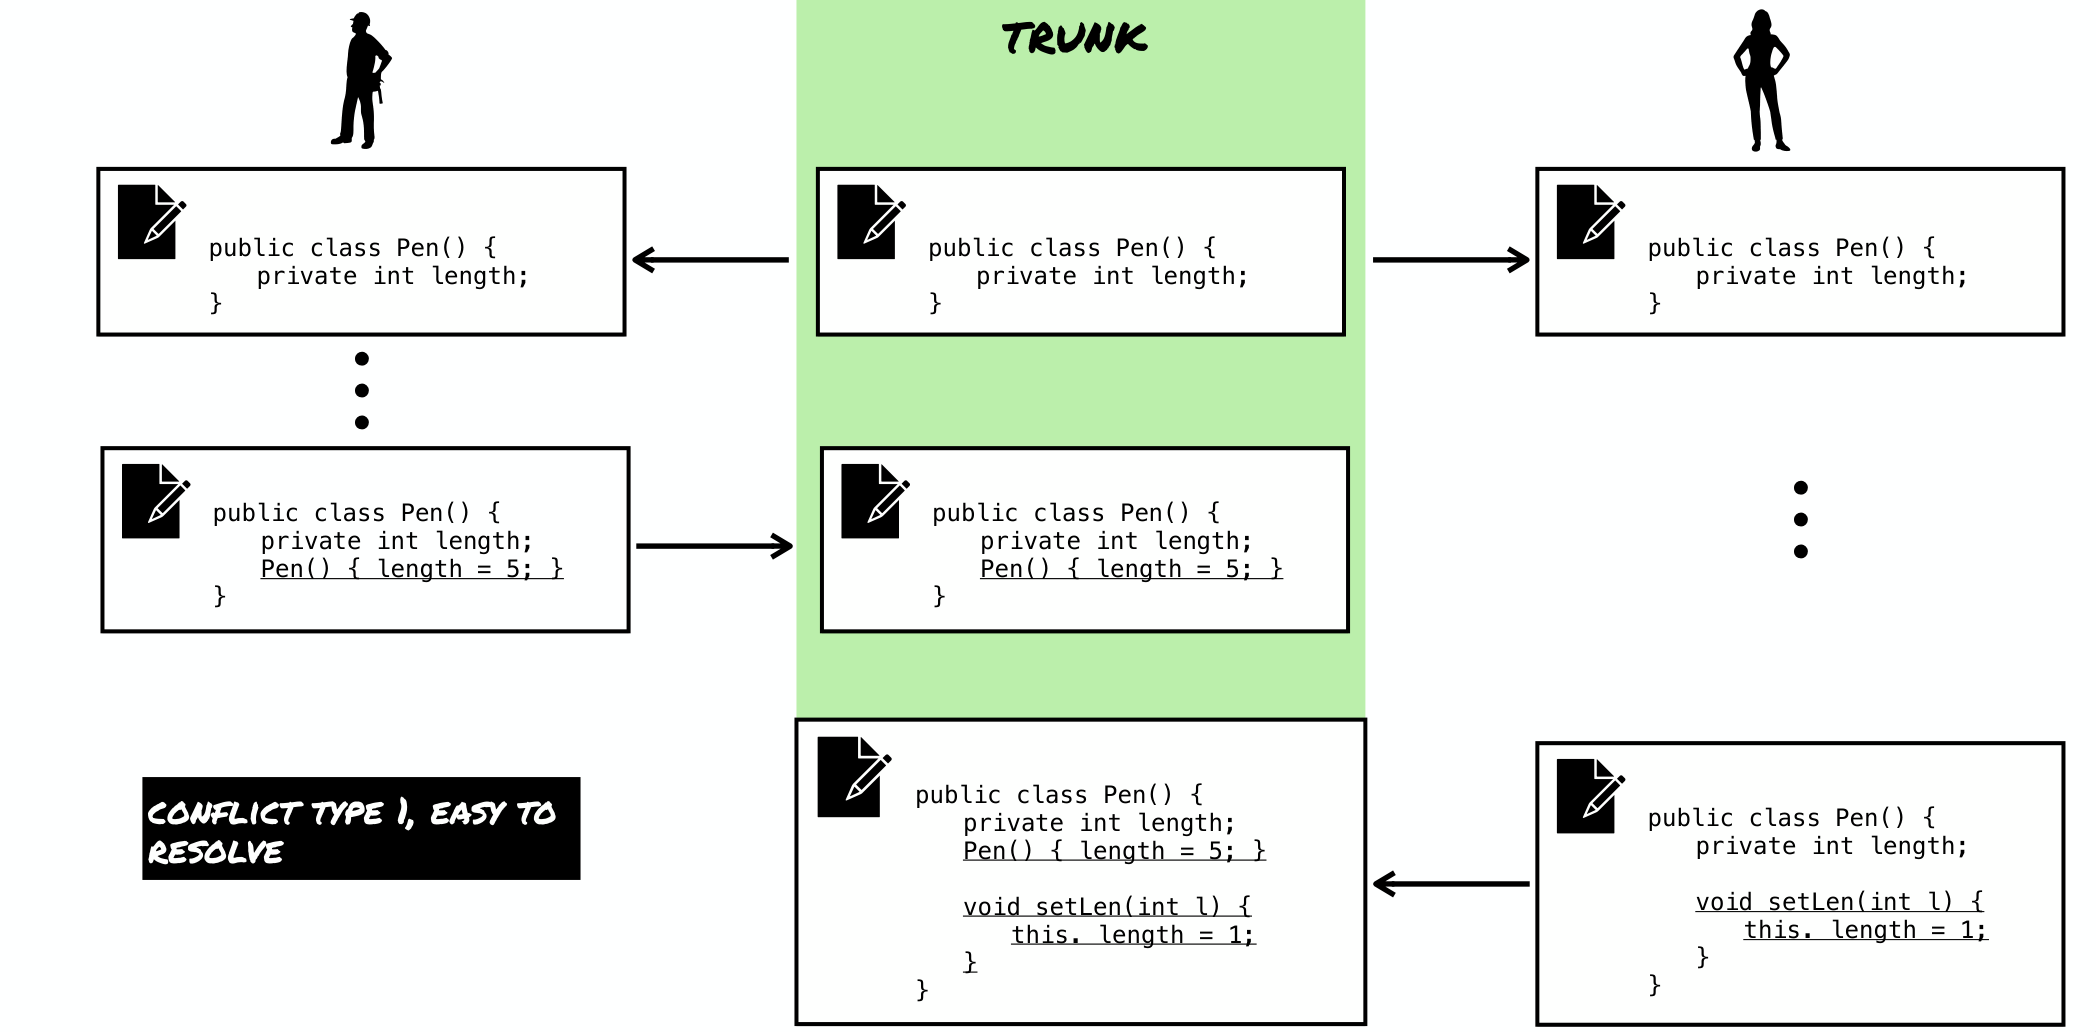
\includegraphics[width=0.8\textwidth]{images/svn_conflict1.png}
    \caption{Type 1 Merge Conflict in Subversion}
\end{figure}

\begin{figure}[H]
    \centering
    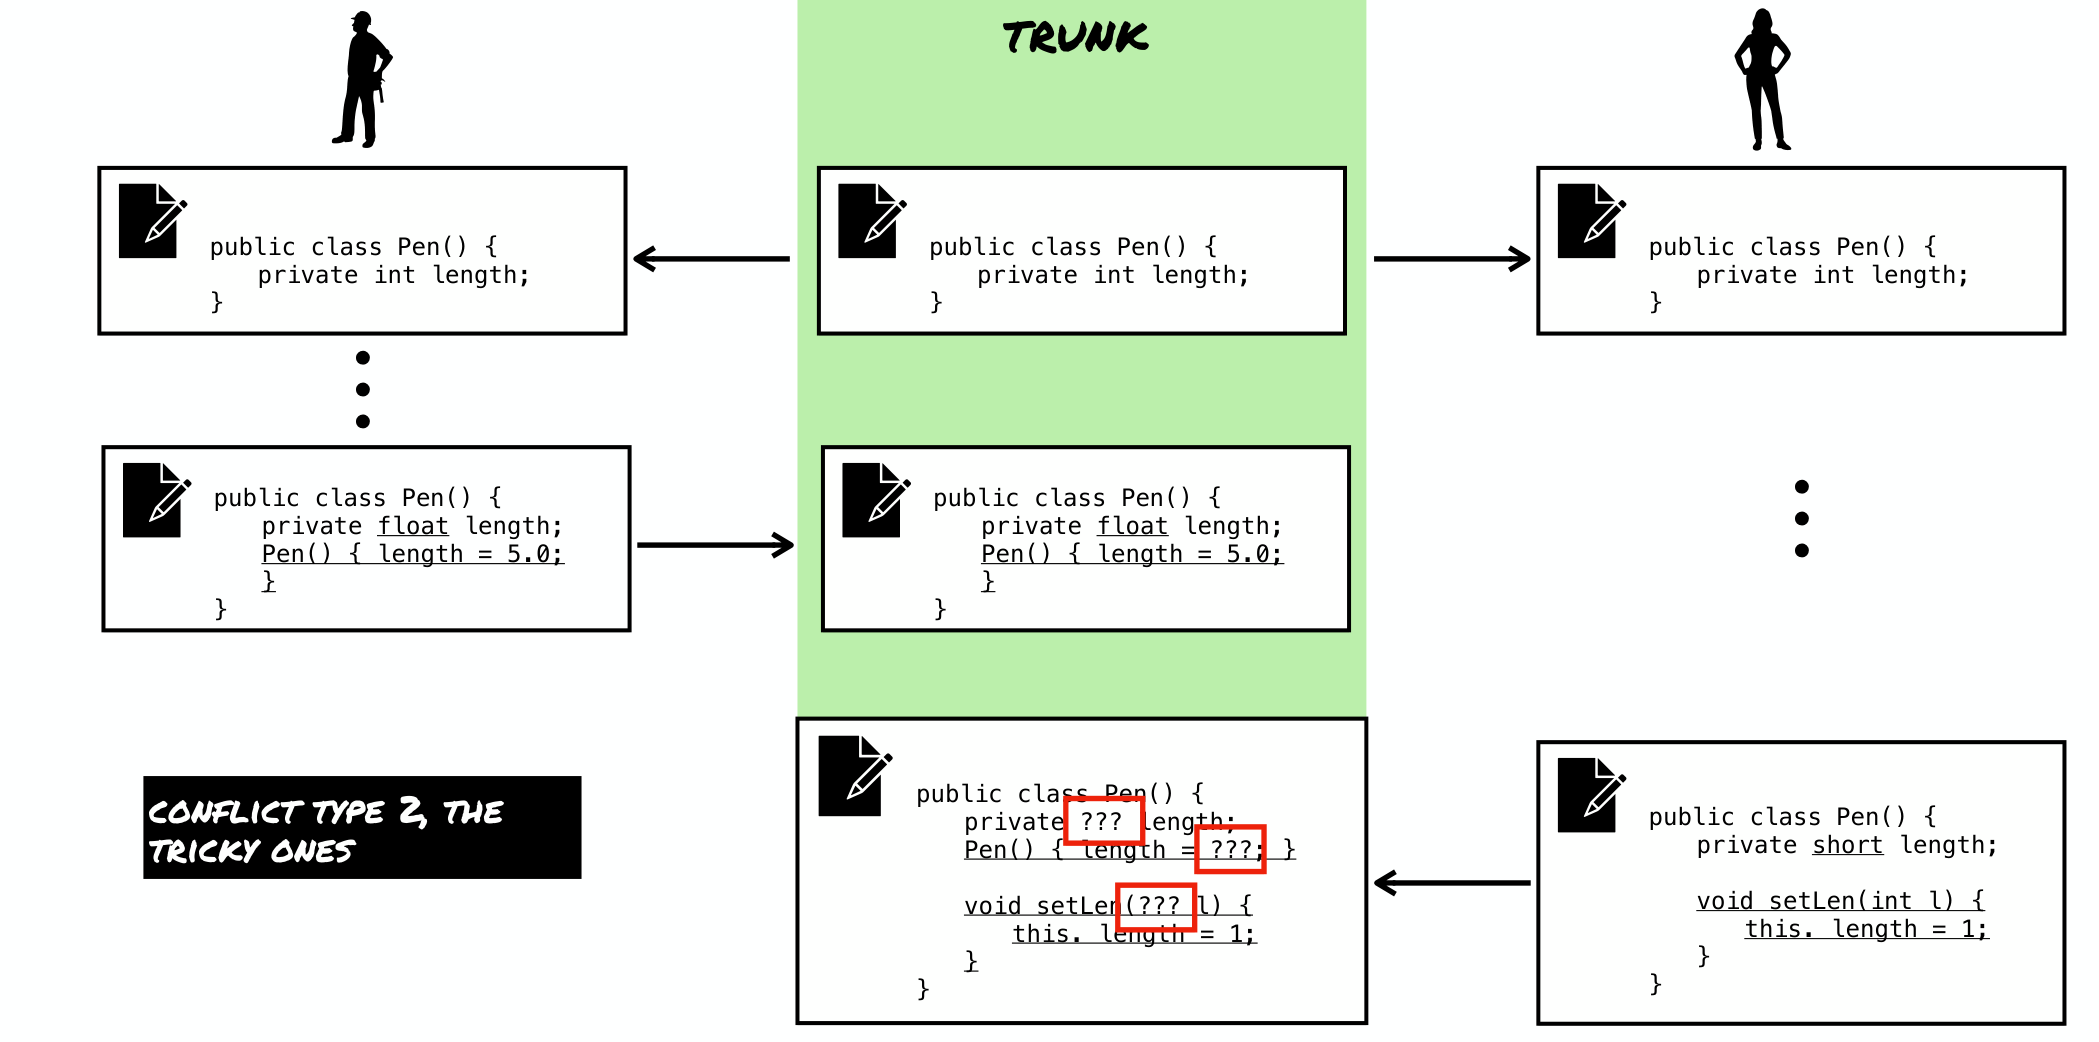
\includegraphics[width=0.8\textwidth]{images/svn_conflict2.png}
    \caption{Type 2 Merge Conflict in Subversion}
\end{figure}

\subsection{Distributed Version Control -- Git}
\begin{figure}[H]
    \centering
    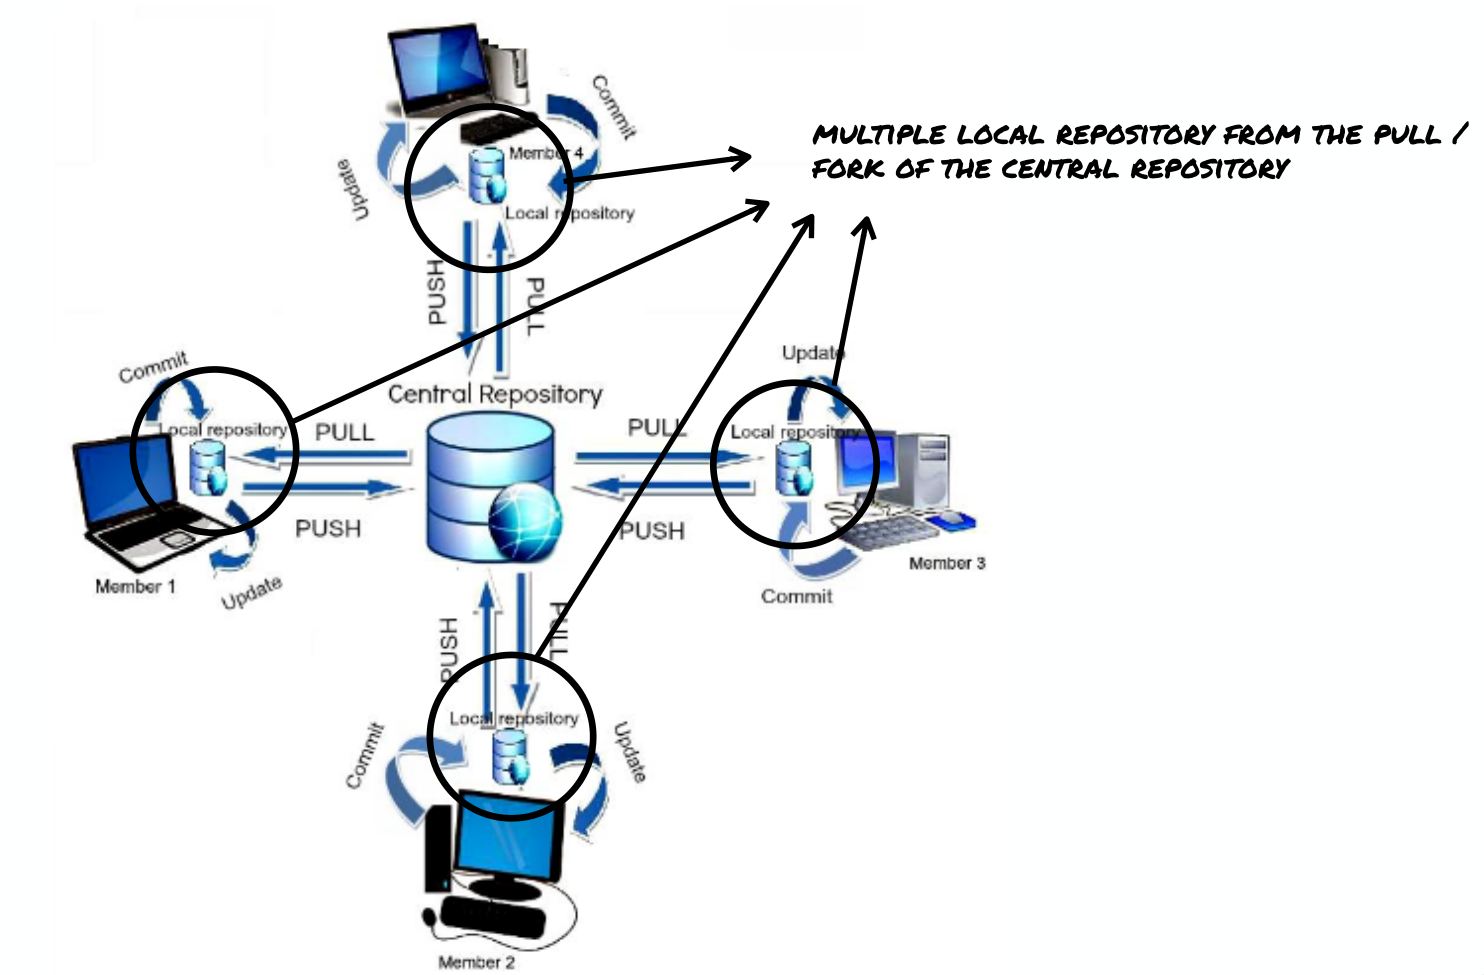
\includegraphics[width=\textwidth]{images/distributed_vcs.png}
    \caption{Distributed Version Control System Diagram}
\end{figure}

Git encourages branching for every feature, regardless of size.
After successful completion of the new feature, the branch is merged into the trunk.
Each developer gets their own local repository, meaning that developers don't need a network connection 
to commit changes, inspect previous version, or compare \verb|diff|s.
If the production trunk / branch is broken, developers can continue working uninhibited.

\subsubsection{GitHub}
\textbf{GitHub} is a web-based hosted service for Git repositories.
It allows you to host remote Git repositories and has a wealth of community-based services that makes it ideal for open-source projects.
It is a publishing tool, a version control system, \& a collaboration platform.

\subsubsection{Git Commands}
\begin{itemize}
    \item   \mintinline{shell}{git clone}: download (``clone'') the source code from the remote repository.
    \item   \mintinline{shell}{git fetch}: fetches the latest version from the repository that you've cloned but doesn't synchronise with all commits
            in the repository.
    \item   \mintinline{shell}{git pull}: pulls the latest version from the repository that you've cloned and synchronises with all commits
            in the repository. Equivalent to running \mintinline{shell}{git fetch} \& \mintinline{shell}{git merge}.
    \item   \mintinline{shell}{git push}: pushes the changes that you have committed to your local branch to the remote repository.
\end{itemize}

\subsubsection{Pull Requests}
A \textbf{pull request} is when you ask another developer to merge your feature branch into their repository.
Everyone can review the code \& decide whether or not it should be included in the master branch.
The pull request is an invitation to discuss pulling your code into the master branch, i.e. it is a forum for discussing changes.

\section{Build Tools}
\begin{figure}[H]
    \centering
    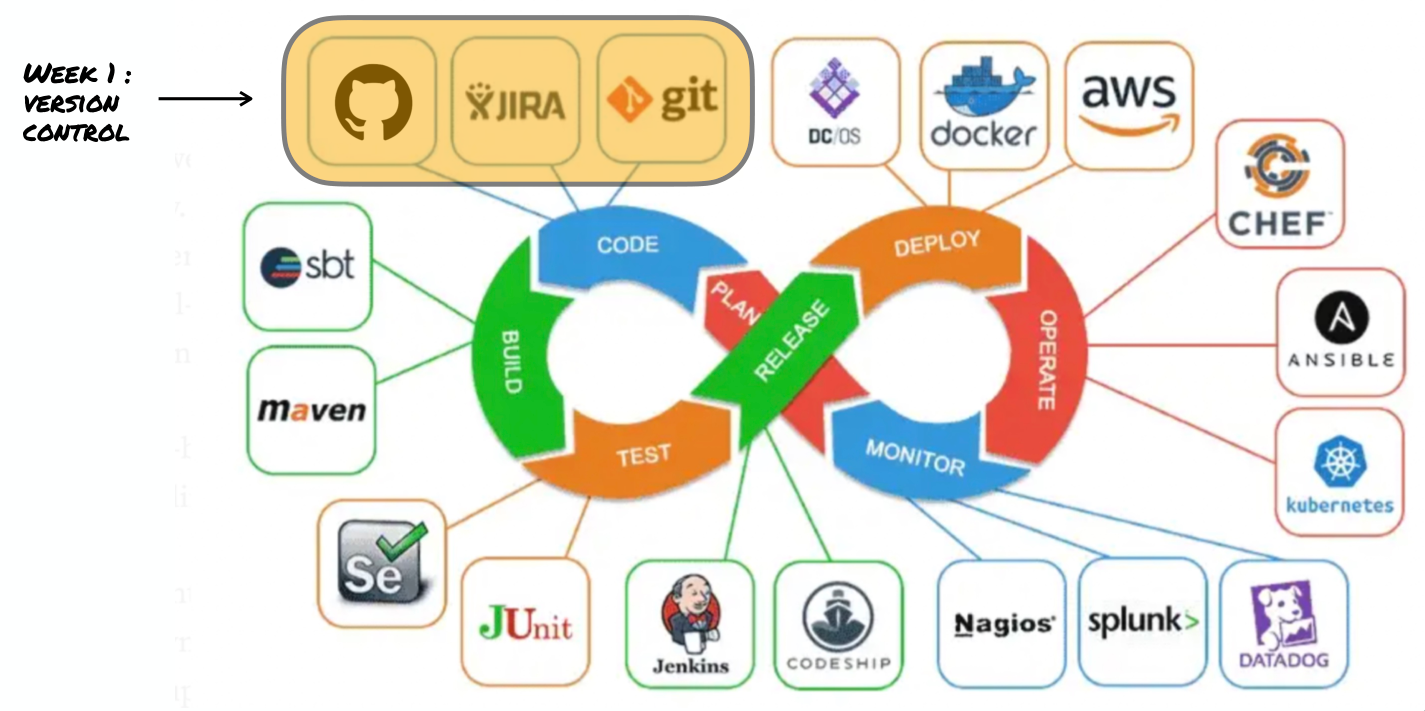
\includegraphics[width=\textwidth]{images/example_cd.png}
    \caption{Example of a Continuous Software Development System}
\end{figure}

The \textbf{build} is a process which covers all the steps required to create a deliverable of your software.
E.g., in Java:
\begin{enumerate}
    \item   Generating sources.
    \item   Compiling sources.
    \item   Compiling test sources.
    \item   Executing tests.
    \item   Packaging (\verb|.JAR|, \verb|.WAR|, \verb|EJB|).
    \item   Running health checks.
    \item   Generating reports.
\end{enumerate}

\textbf{Build tools} are software utilities that automate the tasks of compiling, linking, \& packaging source code into 
executable application or libraries.
Build tools help with:
\begin{itemize}
    \item   \textbf{Automation:} build tools help to automate repetitive tasks such as compiling code, running tests, 
            packaging binaries, \& even deploying applications.
    \item   \textbf{Consistency:} build tools ensure that every build process (e.g., dev, test, prod) is identical, 
            minimising human error.
    \item   \textbf{Efficiency:} build tools speed up development by automating builds whenever code is pushed or merged 
            into a repository.
\end{itemize}

Popular build tools include:
\begin{itemize}
    \item   \textbf{Maven} is a software build tool which can manage the project build, reporting, \& documentation,
            primarily used for Java development and supported by most Java IDEs.
            It features dependency management, project structure standardisation, \& automatic builds.
    \item   \textbf{Gradle} is a build tool that supports multiple languages including Java, Kotlin, \& Groovy.
            Its features include being highly customisable and being faster than Maven due to its incremental builds \&
            caching.
            It's preferred for modern Java-based CI/CD pipelines and supports both Android \& general Java applications.
    \item   \textbf{Node Package Manager (NPM)} is a build tool for JavaScript / Node.js that features dependency 
            management \& building for JavaScript applications.
            It is used to build web-based frontend applications or backend applications in a CI/CD pipeline.
\end{itemize}

Other popular build tools include Yarn for JavaScript, PyBuilder or tox for Python, MSBuild for C\#/.NET, \& Rake for Ruby.

\subsection{Build Tools in CI/CD Pipelines}
\textbf{Continuous Integration (CI)} automatically integrates \& tests code on each commit.
\textbf{Continuous Deployment/Delivery (CD)} automatically deploys tested code to production or staging.
Build tools serve many roles in CI/CD pipelines:
\begin{itemize}
    \item   \textbf{Integration:} when changes are pushed to the repository, the CI tool (e.g., GitHub Actions) triggers the
            build tool to compile \& package the application.
    \item   \textbf{Build Automation:} the build tool automatically handles downloading dependencies, compiling the code, 
            \& running tests.
            It ensures that the same version of the application is built every time.
    \item   \textbf{Testing:} many build tools, such as Maven, integrate with testing frameworks (e.g., JUnit, Selenium) to
            run automated tests after the build.
    \item   \textbf{Deployment:} the packaged application can be deployed to a server, containerised (e.g., with Docker),
            or distributed using CD tools.
\end{itemize}

Build tools automate the process of building \& testing code with each integration to the repository, i.e.
\textbf{Continuous Integration}.
They ensure new changes don't break existing code by running automated tests as part of the build process and exhibit 
\textit{fail-fast} behaviour: if a test or build fails, the developer is notified immediately.
\\\\
After a successful build \& testing, the build tools package the code, ready for deployment, i.e. 
\textbf{Continuous Deployment}.
\textbf{Artifact creation} is when the builds create deployable artifacts (e.g., JAR files, WAR files, Docker images).
The pipeline can then engage in \textbf{automated deployment} by deploying the artifact to a server, cloud, or container.
\\\\
An example build tool workflow in a CI/CD pipeline with GitHub Actions may look like the following:
\begin{enumerate}
    \item   \textbf{Code Push:} a developer pushes new code to the GitHub repository.
    \item   \textbf{CI Tool Trigger:} GitHub Actions detects the change and triggers the pipeline.
    \item   \textbf{Dependency Resolution:} the build tool (e.g., Maven) fetches dependencies from repositories.
    \item   \textbf{Compile \& Build:} the build tool compiles \& packages the code into executable binaries (e.g., JAR, WAR).
    \item   \textbf{Testing:} run unit \& integration tests automatically.
    \item   \textbf{Package \& Deploy:} the build tool creates the package, and the CI/CD pipeline deploys it to staging or 
            production.
\end{enumerate}

\subsection{Maven}
\textbf{Maven} is a software build tool which can manage the project build, reporting, \& documentation, primarily used for
Java development and supported by most Java IDEs.
It is widely used in Spring Boot projects.
\begin{enumerate}
    \item   Compile source code.
    \item   Copy resources.
    \item   Compile \& run tests.
    \item   Package projects.
    \item   Deploy project.
    \item   Cleanup files.
\end{enumerate}

Developers wanted:
\begin{itemize}
    \item   to make the build process easy.
    \item   a standard way to build projects.
    \item   a clear definition of what the project consists of.
    \item   an easy way to publish project information and a way to share JARs across several projects.
\end{itemize}

The result is a tool that developers can use to build \& manage any Java-based project.
It embraces the idea of ``convention over configurations''.

\begin{figure}[H]
    \centering
    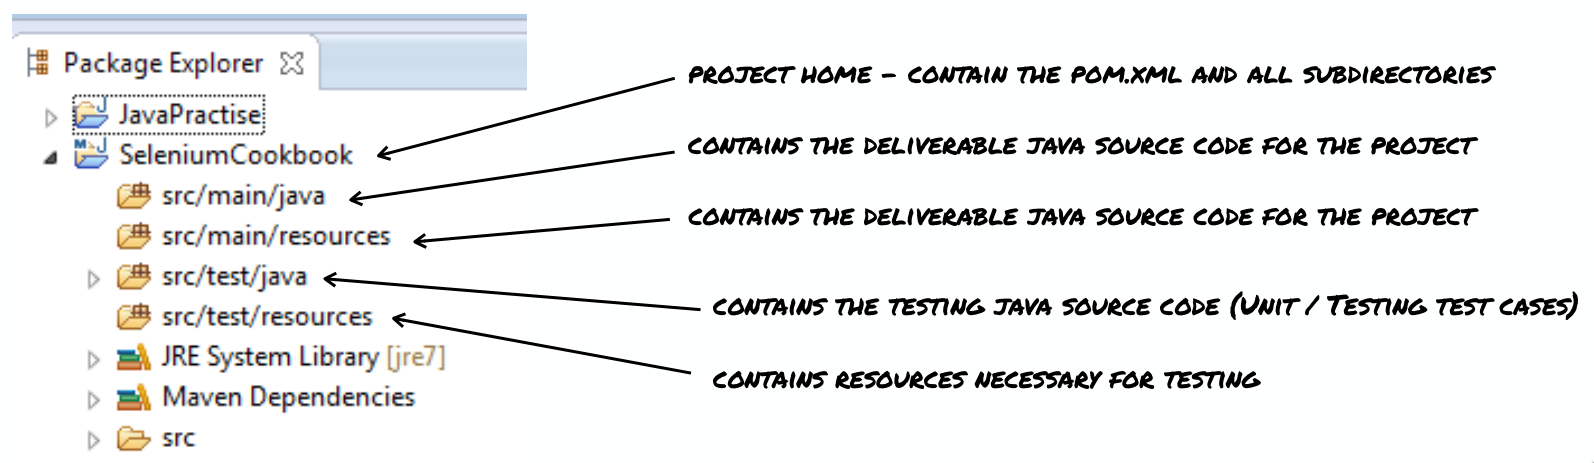
\includegraphics[width=\textwidth]{images/mvn_dir_structure.png}
    \caption{Maven Default Directory Structure}
\end{figure}

The command \mintinline{shell}{mvn package} compiles all the Java files, runs any tests, and packages the 
deliverable code \& resources into \verb|target/my-app-1.0.jar**|.
\\\\
The \verb|pom.xml| file is an XML document that contains all the information that Maven requires to automate 
a build of your software.
The \verb|pom.xml| is automatically updated on demand, but can be manually configured as well.
The POM provides all the configuration for a single project:
\begin{itemize}
    \item   General configuration covers the project's name, its owner, \& its dependencies to other projects.
    \item   One can also configure individual phases of the build process, which are implemented as plugins.
            E.g., one can configure the \verb|compiler-plugin| to use Java 1.5 for compilation, or specify
            packaging the project even if some unit tests fail.
\end{itemize}

Larger projects should be divided into several modules, or sub-projects each with its own POM.
All root POM can compile all the modules with a single command.
POMs can also inherit configuration from other POMs; all POMs inherit from the super-POM by default.
The super-POM provides default configuration, such as default source, default directories, default plugins,
etc.

\subsubsection{Plugins}
Maven build projects based on convention; it expects files to be in a certain place, which is very useful 
when developing in teams.

\begin{figure}[H]
    \centering
    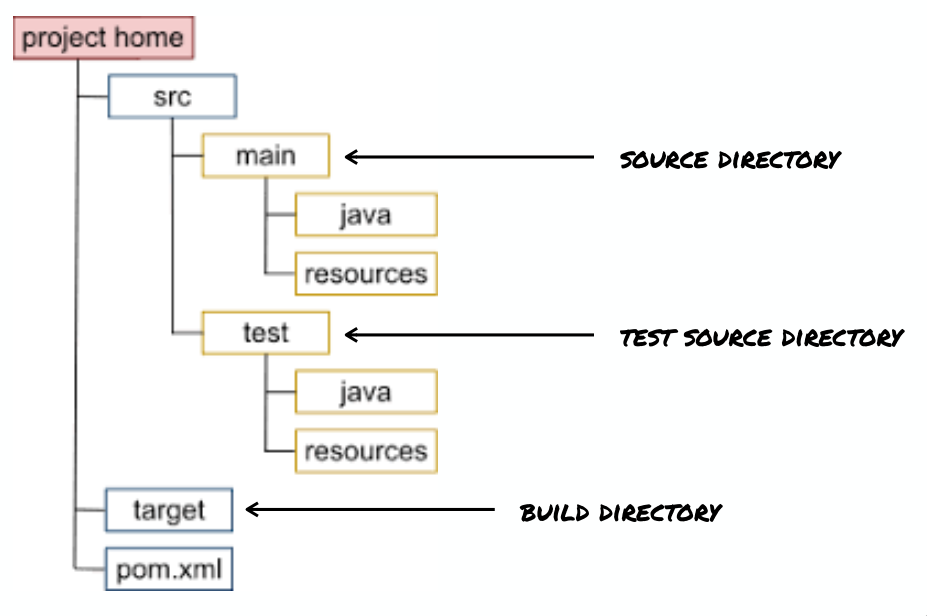
\includegraphics[width=0.7\textwidth]{images/mvn_conv_dir_structure.png}
    \caption{Maven Conventional Directory Structure}
\end{figure}

\begin{figure}[H]
    \centering
    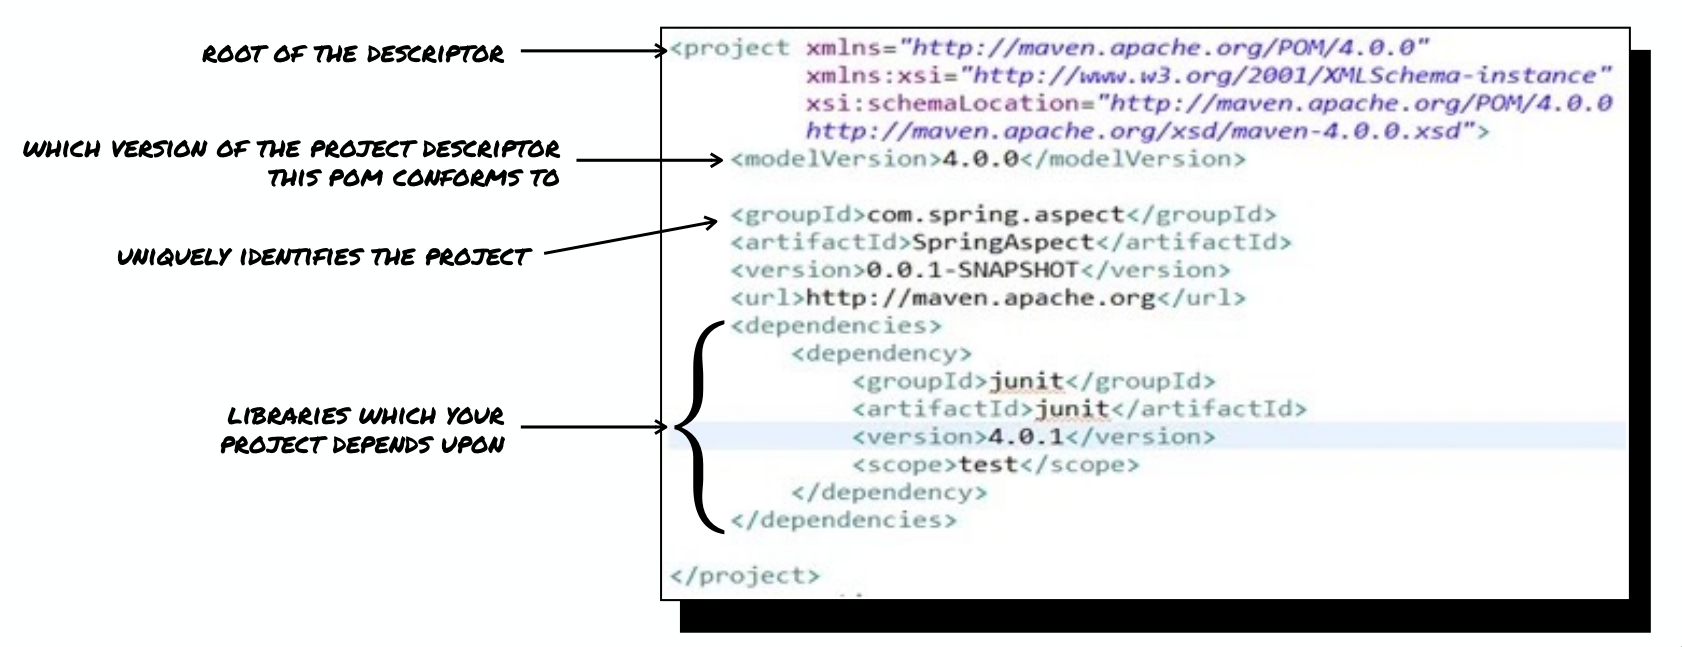
\includegraphics[width=\textwidth]{images/mvn_pom.png}
    \caption{Maven \texttt{pom.xml}}
\end{figure}

A Maven \textbf{plugin} is an extension or add-on module that enhances the functionality of Apache Maven.
Maven plugins provide additional capabilities \& tasks that can be executed during the build process or as part of 
project lifecycle management.
These plugins are typically packages as JAR (Java Archive) files and can be easily added to a Maven project's
configuration.
\\\\
The \textbf{core plugins} are plugins corresponding to default core phases (e.g., clean, compile).
They may also have multiple goals.

\subsubsection{Build Lifecycle}
The process for building \& distributing a particular project is clearly defined. 
It comprises a list of named phases that can be used to give order to goal execution.
Goals provided by plugins can be associated with different phases of the lifecycle.
e.g., by default, the goal \verb|compiler:compile| is associated with the compile phase, while the goal
\verb|surefire:test| is associated with the test phase.
\mintinline{shell}{mvn test} will cause Maven to run all goals associated with each of the phases up to \& including
the test phase.

\subsubsection{Dependency Management}
\textbf{Dependency management} is a central feature in Maven.
The dependency mechanism is organised around a co-ordinate system identifying individual artefacts such as software 
libraries or modules (e.g., JUnit).
If your project depends on a JAR file, Maven will automatically retrieve it for you, and store it in the user's local
repository.
If the JAR file depends on other libraries, Maven will ensure these are also included: these are known as 
\textbf{transitive dependencies}.
This wasn't always a part of Maven, so it's a huge benefit.
\\\\
Dependency management features supported include:
\begin{itemize}
    \item   Management: you can specify library version that transitive dependencies should use.
    \item   Scope: include dependencies appropriate for the current stage of the build, i.e., compile, test, run, etc.
    \item   Exclude dependencies: if project X depends on Project Y, and Project Y depends on Project Z, you can choose
            to exclude Project Z from your build.
\end{itemize}

\subsubsection{Local \& Remote Repository}
The remote repository \url{https://mvnrepository.com/} contains libraries for almost everything: cloud computing,
date \& time utilities, HTML parsers, mail clients, etc.
Once you specify the correct details in the POM file, Maven will automatically fetch the library for you on build.
\\\\
The local Maven repository can be found at \verb|~/.m2/|.
Maven will search the local repository first and then search third-party repositories if it does not find what it's looking
for.
You can create your own repository and share it within your organisation.

\subsection{Spring Boot}
\textbf{Spring Boot} is a framework for building standalone Java applications with embedded servers that streamlines Java
application development.
It provides pre-configured, out-of-the-box functionality to avoid boilerplate code.
It reduces configuration \& setup, focuses on \textit{convention over configuration}, and is compatible with microservices
architecture, REST APIs, \& monolithic apps.

\subsubsection{Spring vs Spring Boot}
\textbf{Spring} is a comprehensive framework for building any Java application requiring more manual configuration \& 
management of dependencies \& application context.
Spring Boot is an extension of the Spring framework aimed at simplifying development, configuration, \& deployment, 
especially for microservices \& cloud-based applications.

\begin{table}[h!]
    \centering

    \begin{tabular}{|>{\arraybackslash}p{0.5\textwidth}|>{\arraybackslash}p{0.5\textwidth}|}
        \hline
        \textbf{Spring}                                                 & \textbf{Spring Boot} \\
        \hline
        Requires an external embedded server (e.g, Tomcat, Jetty, etc.) & Comes with an embedded server (Tomcat/Jetty)\\
        \hline
        Highly flexible but requires more setup effort                  & Simplifies Spring projects, reducing setup time \\
        \hline
        Best for complex, large-scale applications                      & Ideal for microservices \& fast prototypes \\
        \hline
        Requires WAR file and deployment on external server             & Packaged as JAR with an embedded server for easy deployment \\
        \hline
    \end{tabular}
    \caption{Technical Differences between Spring \& Spring Boot}
\end{table}

Choose Spring when:
\begin{itemize}
    \item   Your project requires extensive customisations.
    \item   You're building a complex enterprise application where flexibility \& modularity are necessary.
    \item   You have a team experiences in managing detailed configurations.
\end{itemize}

Choose Spring Boot when:
\begin{itemize}
    \item   You're building microservices or need quick iterations in development.
    \item   You want an all-in-one solution with auto-configuration.
    \item   Your focus is on simplicity \& speed without worrying about configuration details.
\end{itemize}

\begin{table}[h!]
    \centering

    \begin{tabular}{|>{\arraybackslash}p{0.5\textwidth}|>{\arraybackslash}p{0.5\textwidth}|}
        \hline
        \textbf{Spring}                                                     & \textbf{Spring Boot} \\
        \hline
        Framework for building complex enterprise-level Java applications   & Simplified framework to quickly build microservices or standalone apps \\
        \hline
        Slower to set up due to configuration                               & Faster development with minimal setup \\
        \hline
        Provides maximum flexibility \& customisation                       & Less flexibility, focuses on ease of use \\
        \hline
        Suitable for large-scale, complex, highly customised apps           & Suitable for small/medium projects, microservices, \& rapid development \\
        \hline
    \end{tabular}
    \caption{High-Level Differences between Spring \& Spring Boot}
\end{table}

\subsection{GitHub Actions}
\textbf{GitHub Actions} automates your workflow by triggering events such as \verb|push|, \verb|pull_request|, \&
\verb|release|.
It easily integrates with other tools like Docker, AWS, Heroku, etc.
Key components of GitHub Actions include:
\begin{itemize}
    \item   \textbf{Workflows} are defined in YAML in the \verb|.github/workflows/| folder and are triggered by events such 
            as \verb|push|, \verb|pull_request|, etc.
    \item   \textbf{Jobs} define units of work that run on a \textbf{runner} (e.g., \verb|ubuntu_latest|,
            \verb|macos-latest|).
            They can be run sequentially or in parallel.
    \item   Each job consists of a series of \textbf{steps}, e.g., checking out the code, building, testing, etc.
    \item   \textbf{Runners} include GitHub-hosted runners (e.g., Ubuntu, macOS) but you can also have self-hosted runners 
            to run on your own infrastructure.
    \item   \textbf{GitHub Secrets} can be used to securely store sensitive information (e.g., API keys) and are accessible 
            in workflows as \mintinline{yaml}{secrets.MY_SECRET_KEY}.
\end{itemize}

\textbf{Composite actions} can be used to define reusable workflows.

\section{Containerisation}
\textbf{Containerisation} is a method of packaging software \& all of its dependencies so that it can run
uniformly \& consistently across any infrastructure.
Containers are isolated environments in which applications run, ensuring consistent behaviour across different
environments (e.g., development, testing, production).

\begin{figure}[H]
    \centering 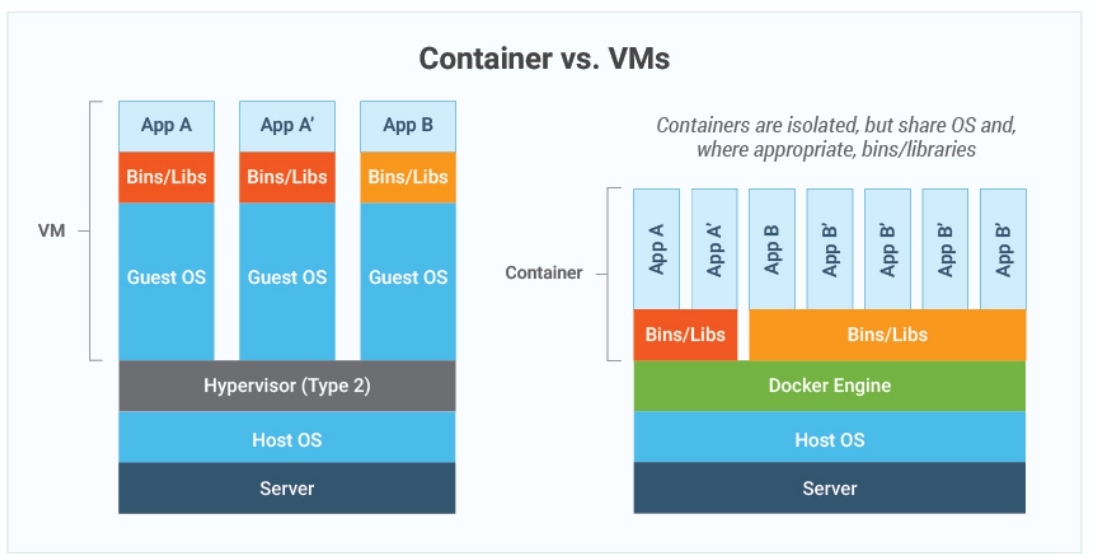
\includegraphics[width=\textwidth]{images/containers_vs_vms.png}
    \caption{Virtual Machines vs Containers }
\end{figure}

Containers virtualise the operating system, while virtual machines virtualise the hardware.
Containers share the OS kernel but isolate the application \& its dependencies.

\begin{table}[h!]
    \centering

    \begin{tabular}{|>{\arraybackslash}p{0.5\textwidth}|>{\arraybackslash}p{0.5\textwidth}|}
        \hline
        \textbf{Virtual Machines}                                           & \textbf{Containers} \\
        \hline
        Heavy \& resource-intensive                                         & Lightweight, share the OS kernel \\
        \hline
        Requires an entire OS for each VM                                   & Faster startup, less overhead \\
        \hline
        Slower startup \& resource usage                                    & More efficient resource usage\\
        \hline
    \end{tabular}
    \caption{Virtual Machines vs Containers}
\end{table}

Reasons for using containerisation include:
\begin{itemize}
    \item   \textbf{Portability:} containers ensure that applications run the same regardless of the environment.
    \item   \textbf{Scalability:} containers can be scaled easily, making them ideal for microservice architectures.
    \item   \textbf{Efficiency:} containers are lightweight and use fewer resources than traditional VMs.
    \item   \textbf{Isolation:} each container is isolated, meaning multiple containers can run on the same host
            without interference.
    \item   \textbf{Faster deployment:} containers can be started in seconds, enabling fast deployments \& rollbacks.
\end{itemize}

\subsection{Docker}
\textbf{Docker} is an open-source platform for building, deploying, \& managing containerised applications.
It simplifies container creation \& management, and provides a consistent environment for development, testing, \&
production.
Advantages of using Docker include:
\begin{itemize}
    \item   \textbf{Consistency across environments:} Docker ensures that the application runs the same regardless
            of where it's deployed.
            Eliminates the ``works on my machine'' problem by providing a consistent environment across all 
            stages of development.
    \item   \textbf{Isolation:} containers provide process isolation, so multiple applications or microservices can
            run side-by-side without interfering with each other.
    \item   \textbf{Scalability:} containers are lightweight and can be easily scaled horizontally (i.e., 
            replicating containers to handle more traffic).
    \item   \textbf{Efficiency:} compared to virtual machines, containers use fewer resources since they share
            the host machine's kernel, making them much faster to start and stop.
    \item   \textbf{Portability:} applications packaged in Docker containers can be easily moved across
            environments, cloud platforms, \& OSes, ensuring smooth \& reliable deployments.
    \item   \textbf{Easy integration:} seamlessly integrates with CI/CD tools \& workflows.
\end{itemize}

Key terms in Docker include:
\begin{itemize}
    \item   \textbf{Image:} a lightweight, standalone, executable package that includes everything an application 
            needs (code, runtime, libraries, dependencies).
    \item   \textbf{Container:} a runtime instance of an image.
            While images are static, containers are dynamic and can be started, stopped, or moved across environments.
    \item   \textbf{Dockerfile:} a text file with instructions to build a docker image.
            It defines the steps to configure an environment, install dependencies, and set up the application.
    \item   \textbf{Docker Hub:} a cloud-based repository for finding \& sharing container images, both public \&
            private.
\end{itemize}

\begin{figure}[H]
    \centering 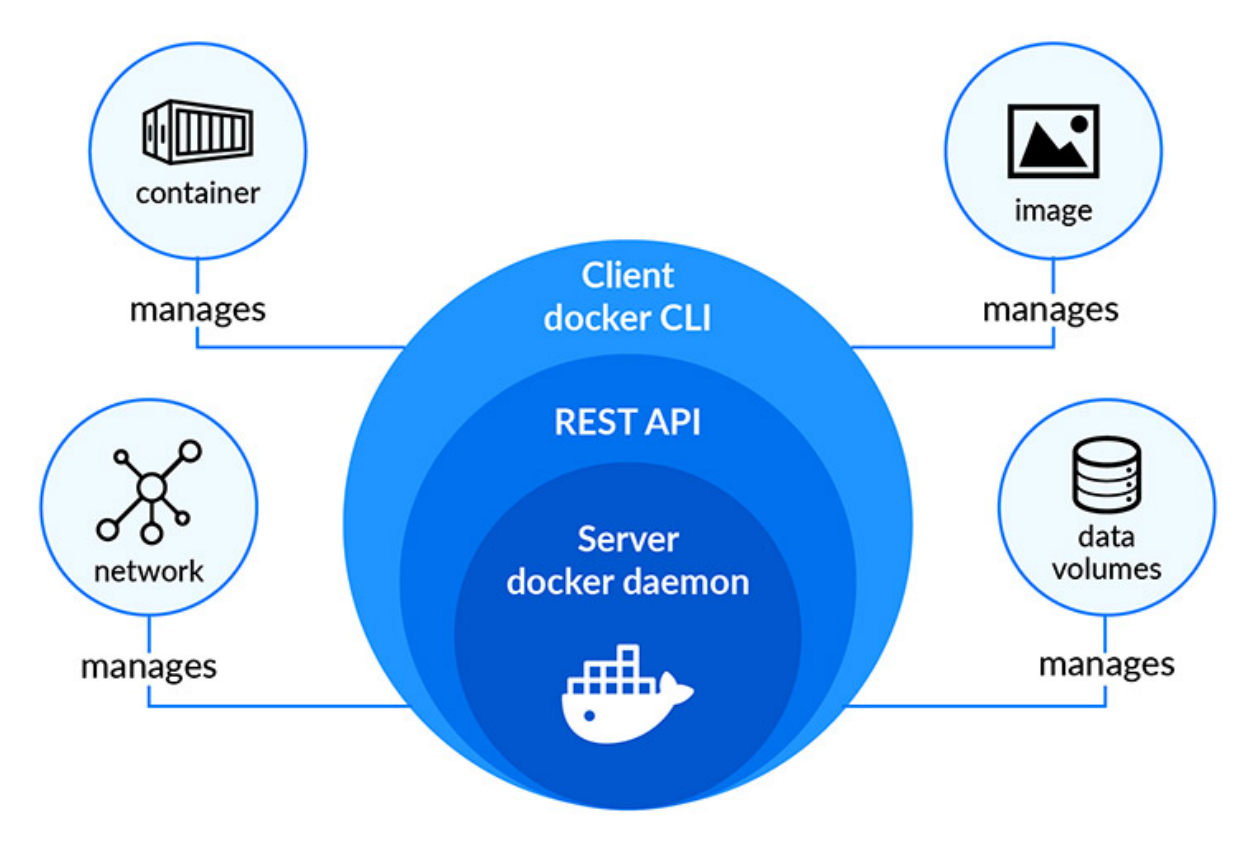
\includegraphics[width=\textwidth]{images/docker_overview.png}
    \caption{Docker Architecture Overview}
\end{figure}

Key Docker components include:
\begin{itemize}
    \item   \textbf{Docker Engine:} the runtime that runs \& manages containers.
    \item   \textbf{Docker Hub:} a public repository where users can publish \& share container images.
    \item   \textbf{Dockerfile:} a text files that contains instructions on how to build a Docker image.
\end{itemize}

\subsubsection{Building \& Running Applications in Docker Containers}
The dockerfile structure is as follows:
\begin{itemize}
    \item   \mintinline{dockerfile}{FROM}: the base image (e.g., \verb|openjdk:17| for Java applications).
    \item   \mintinline{dockerfile}{WORKDIR}: the directory inside the container where the application will reside.
    \item   \mintinline{dockerfile}{COPY}: copies files from the host system into the container.
    \item   \mintinline{dockerfile}{RUN}: executes commands (e.g., installing dependencies).
    \item   \mintinline{dockerfile}{CMD}: defines the default command to run when the container starts (e.g., 
            \mintinline{shell}{java -jar app.jar}).
\end{itemize}

\begin{code}
\begin{minted}[linenos, breaklines, frame=single]{dockerfile}
FROM openjdk:17-jdk-slim
WORKDIR /app
COPY target/musicFinder-1.0 jar app.jar
EXPOSE 8080
ENTRYPOINT ["java", "-jar", "app.jar"]
\end{minted}
\caption{Example Dockerfile for a Spring Boot Application}
\end{code}

To build the Docker image from the Dockerfile:
\begin{minted}[linenos, breaklines, frame=single]{shell}
docker build -t my-app .
\end{minted}

The Docker container can then be run, mapping the container's port 8080 to the host's port 8080:
\begin{minted}[linenos, breaklines, frame=single]{shell}
docker run -p 8080:8080 my-app
\end{minted}

\subsubsection{Docker Best Practices}
\begin{itemize}
    \item   \textbf{Keep images lightweight:} use minimal base images (e.g., \verb|alpine|) to reduce the size of 
            the final image, leading to faster build times \& fewer security vulnerabilities.
    \item   \textbf{Multi-stage builds:} separate the build environment from the final image to reduce size \&
            improve performance.
            \begin{minted}[linenos, breaklines, frame=single]{dockerfile}
FROM maven:3.8-jdk-11 AS builder
WORKDIR /build
COPY . .
RUN mvn clean package

FROM openjdk:11-jre-slim
WORKDIR /app
COPY --from=builder /build/target/app.jar /app.jar
CMD ["java", "-jar", "/app.jar"]
            \end{minted}

    \item   \textbf{Use \texttt{.dockerignore}:} similar to \verb|.gitignore|, it prevents unnecessary files from
            being copied into the container, optimising build times.

    \item   \textbf{Tagging:} tag your images \mintinline{shell}{docker build -t my-app:v1} for version control \&
            easier management of deployments.

    \item   Security best practices include:
            \begin{itemize}
                \item   Regularly update base images to avoid security vulnerabilities.
                \item   Avoid running containers as root.
                \item   Scan your Docker images for vulnerabilities using tools like Clair or Anchore.
            \end{itemize}
\end{itemize}

\subsubsection{Common Docker Commands}
\begin{itemize}
    \item   Listing containers:
            \begin{itemize}
                \item   \mintinline{shell}{docker ps}: list running containers.
                \item   \mintinline{shell}{docker ps -a}: list all containers, including stopped ones.
            \end{itemize}

    \item   Stopping / removing containers:
            \begin{itemize}
                \item   \mintinline{shell}{docker stop container_id}: stops a running container.
                \item   \mintinline{shell}{docker rm container_id}: removes a stopped container.
            \end{itemize}

    \item   Viewing logs:
            \begin{itemize}
                \item   \mintinline{shell}{docker logs container_id}: shows the logs of a container.
            \end{itemize}

    \item   Entering a running container:
            \begin{itemize}
                \item   \mintinline{shell}{docker exec -it container_id /bin/bash}: opens a shell inside the running
                        container.
            \end{itemize}
\end{itemize}

\begin{figure}[H]
    \centering 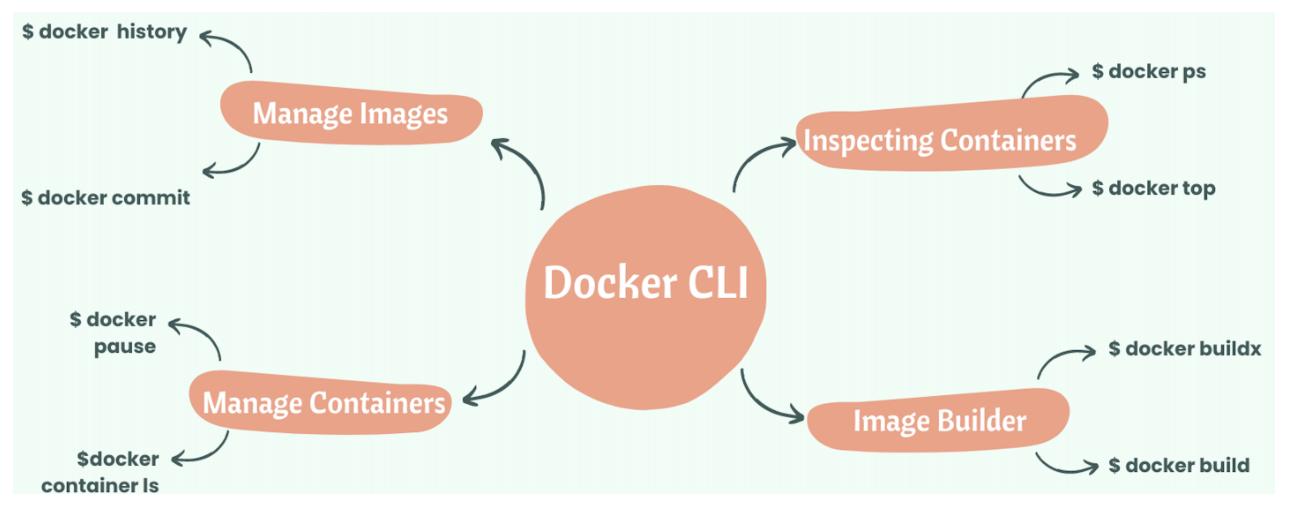
\includegraphics[width=\textwidth]{images/common_docker_cmds.png}
    \caption{Some Common Docker Commands}
\end{figure}

\subsubsection{Practical Docker Example with Spring Boot}
Prerequisites:
\begin{itemize}
    \item   Java 17 SDK.
    \item   Docker (running).
    \item   Maven.
    \item   Sprint Boot CLI (Optional, but useful for scaffolding projects).
\end{itemize}

\begin{enumerate}
    \item   Initialise a Spring Boot project with Maven using Spring Initializr to generate the project structure.
    \item   Create the Song Suggester Logic in \verb|src/main/java/com/example/songsuggester/SongSuggesterController.java|:
            \begin{minted}[linenos, breaklines, frame=single]{dockerfile}
package com.example.songsuggester;

import org.springframework.web.bind.annotation.GetMapping;
import org.springframework.web.bind.annotation.RestController;
import org.springframework.web.client.RestTemplate;
import org.json.JSONObject;
import java.util.Random;

@RestController
public class SongSuggesterController {
    @GetMapping("/suggest")
    public String suggestSong() {
        String apiUrl = "https://itunes.apple.com/search?term=pop&limit=10";
        RestTemplate restTemplate = new RestTemplate();
        String result = restTemplate.getForObject(apiUrl, String.class);

        // Parse the JSON response
        JSONObject jsonObject = new JSONObject(result);
        var tracks = jsonObject.getJSONArray("results");

        // Randomize the selection
        Random rand = new Random();
        int randomIndex = rand.nextInt(tracks.length());
        var randomTrack = tracks.getJSONObject(randomIndex);

        // Extract the song and artist name
        String song = randomTrack.getString("trackName");
        String artist = randomTrack.getString("artistName");

        return "Today's song suggestion: " + song + " by " + artist;
    }
}
            \end{minted}

    \item   Build and run the Spring Boot application:
            \begin{enumerate}[label=\roman*.]
                \item   Navigate to the project folder.
                \item   Run the Maven build command:
                        \begin{minted}[linenos, breaklines, frame=single]{dockerfile}
mvn clean install
                        \end{minted}
                \item   Start the Spring Boot application:
                        \begin{minted}[linenos, breaklines, frame=single]{dockerfile}
mvn spring-boot:run
                        \end{minted}
                \item   Access the application by navigating to \url{http://localhost:8080/suggest} in your browser.
            \end{enumerate}

            \item   In the root of your project directory, create a Dockerfile:
                    \begin{minted}[linenos, breaklines, frame=single]{dockerfile}
# Use an official OpenJDK runtime as a parent image
FROM openjdk:17-jdk-slim

# Set the working directory inside the container
WORKDIR /app

# Copy the project JAR file into the container
COPY target/song-suggester-0.0.1-SNAPSHOT.jar app.jar

# Expose the port the app runs on
EXPOSE 8080

# Run the JAR file
ENTRYPOINT ["java", "-jar", "app.jar"]
                    \end{minted}

    \item   Build the Docker image from the Dockerfile:
            \begin{minted}[linenos, breaklines, frame=single]{shell}
docker build -t song-suggester .
            \end{minted}

    \item   Run the Docker container:
            \begin{minted}[linenos, breaklines, frame=single]{shell}
docker run -p 8080:8080 song-suggester
            \end{minted}
\end{enumerate}

\subsection{Container Orchestration}
\textbf{Container orchestration} automates the management, deployment, scaling, \& networking of containers.
It's crucial when dealing with a large number of containers running across multiple environments because as the
number of containers grows, manually managing them becomes unfeasible.
\\\\
Key components of container orchestration include:
\begin{itemize}
    \item   \textbf{Scheduling:} automatically assigns containers to hots machines based on resource availability.
    \item   \textbf{Scaling:} dynamically adds or removes containers based on demand.
    \item   \textbf{Networking:} manages the communication between containers and ensures that they can interact
            securely.
    \item   \textbf{Load balancing:} distributes traffic across multiple containers to optimise resource usage.
    \item   \textbf{Service discovery:} automatically detects and connects services running in different containers.
\end{itemize}

Orchestration benefits DevOps in the following ways:
\begin{itemize}
    \item   \textbf{Automation:} simplifies repetitive tasks such as deployment, scaling, \& rollback.
    \item   \textbf{High availability:} distributes workloads across different machines, ensuring that services
            remain available.
    \item   \textbf{Fault tolerance:} automatically restarts or replaces failed containers and reroutes traffic
            to healthy containers.
    \item   \textbf{Scalability:} orchestrators can dynamically scale the number of running containers to handle
            increased traffic.
\end{itemize}

Challenges with container orchestration include:
\begin{itemize}
    \item   \textbf{Complexity:} orchestration platforms can introduce signification complexity, especially for
            small teams.
    \item   \textbf{Learning curve:} tools like Kubernetes have a steep learning curve for new users.
    \item   \textbf{Resource overhead:} orchestrators can consume considerable resources, particularly when
            managing large-scale systems.
    \item   \textbf{Networking:} configuring secure \& reliable networking between containers can be challenging.
\end{itemize}

Popular container orchestration tools include:
\begin{itemize}
    \item   \textbf{Kubernetes:}
            \begin{itemize}
                \item   Most widely used container orchestration platform.
                \item   Manages containerised application across clusters of machines.
                \item   Handles self-healing, automated rollouts, \& scaling.
            \end{itemize}
    \item   \textbf{Docker Swarm:}
            \begin{itemize}
                \item   Built-in Docker tool for orchestration.
                \item   Easier to set up but less feature-rich than Kubernetes.
                \item   Ideal for smaller setups with Docker-native capabilities.
            \end{itemize}
    \item   \textbf{Apache Mesos:}
            \begin{itemize}
                \item   General-purpose distributed systems platform that supports container orchestration.
                \item   Suitable for large-scale environments requiring both container \& non-container workloads.
            \end{itemize}
\end{itemize}

\subsubsection{Kubernetes}
The Kubernetes architecture consists of a master node \& worker nodes:
\begin{itemize}
    \item   \textbf{Master Node:} manages the Kubernetes cluster.
            \begin{itemize}
                \item   \textbf{API Server:} entry point for REST operations.
                \item   \textbf{Scheduler:} assigns containers to nodes.
                \item   \textbf{Controller Manager:} ensures the desired state of the system.
            \end{itemize}
    \item   \textbf{Worker Nodes:} hosts running containerised applications.
            \begin{itemize}
                \item   \textbf{Kubelet:} ensures containers are running on a node.
                \item   \textbf{Pod:} smallest deployable unit consisting of one or more containers, with shared
                        storage \& network resources.
                \item   \textbf{Kube-Proxy:} handles networking within Kubernetes.
            \end{itemize}
\end{itemize}

Key Kubernetes concepts include:
\begin{itemize}
    \item   \textbf{Service:} an abstraction that defines a logical set of pods \& a policy for accessing them.
    \item   \textbf{Deployment:} manages pod scaling \& rolling updates for your application.
    \item   \textbf{Namespace:} provides scope for resources within a Kubernetes cluster, helping organise \& 
            manage resources.
\end{itemize}

The steps to run Kubernetes locally are as follows:
\begin{enumerate}
    \item   \textbf{Install Minikube:} Minikube allows you to run Kubernetes on a single node.
            \begin{minted}[linenos, breaklines, frame=single]{shell}
curl -LO https://storage.googleapis.com/minikube/releases/latest/minikube-linux-amd64
sudo install minikube-linux-amd64 /usr/local/bin/minikube
\end{minted}
    \item   Install \verb|kubectl|:
            \begin{minted}[linenos, breaklines, frame=single]{shell}
sudo apt-get install -y apt-transport-https
curl -s https://packages.cloud.google.com/apt/doc/apt-key.gpg | sudo apt-key add -
echo "deb https://apt.kubernetes.io/ kubernetes-xenial main" | sudo tee -a /etc/apt/sources.list.d/kubernetes.list
sudo apt-get update
sudo apt-get install -y kubectl
            \end{minted}
            Verify the installation by running \mintinline{shell}{kubectl version}.
    \item   Running Kubernetes:
            \begin{itemize}
                \item   Use the following commands to start interacting with your Kubernetes cluster:
                \begin{minted}[linenos, breaklines, frame=single]{shell}
kubectl cluster-info
kubectl get nodes
                \end{minted}
                You can deploy containers \& pods using:
                \begin{minted}[linenos, breaklines, frame=single]{shell}
kubectl apply -f <your-deployment-file>.yaml
                \end{minted}
            \end{itemize}
    \item   Manage Kubernetes with Helm (optional):
            \begin{itemize}
                \item   \textbf{Helm} is a package manager for Kubernetes that makes deployment easier.
                \item   To install Helm:
                        \begin{minted}[linenos, breaklines, frame=single]{shell}
curl https://raw.githubusercontent.com/helm/helm/main/scripts/get-helm-3 | bash
                        \end{minted}
                \item   You can then start deploying applications using Helm Charts.
            \end{itemize}
\end{enumerate}

To deploy the \verb|song-suggester| app with Kubernetes:
\begin{enumerate}
    \item   Create a Docker image for the \verb|suggest-music| app:
            \begin{minted}[linenos, breaklines, frame=single]{shell}
docker build -t song-suggester .
            \end{minted}
    \item   Deploy the Docker container in a Kubernetes pod:
            \begin{minted}[linenos, breaklines, frame=single]{shell}
kubectl create deployment song-suggester --image=song-suggester
            \end{minted}
    \item   Expose the app using a service to make it accessible outside the Kubernetes cluster:
            \begin{minted}[linenos, breaklines, frame=single]{shell}
kubectl expose deployment song-suggester -type=LoadBalancer -- port=8080
            \end{minted}
    \item   Scale the application to run multiple instances:
            \begin{minted}[linenos, breaklines, frame=single]{shell}
kubectl scale deployment song-suggester --replicas=5
            \end{minted}
\end{enumerate}

\section{DevSecOps}
Traditional development cycles considered security at the end, leading to costly vulnerabilities in production.
Modern applications involve complex microservices, and frequent releases that increase attack surfaces.
Key risks in modern development include:
\begin{itemize}
    \item   Faster development leads to higher risks; without security baked into the process, vulnerabilities
            can go unnoticed until late stages.
    \item   Complex architectures such as containerised environments \& cloud infrastructure create new attack
            vectors.
    \item   Increasing rates of cyberattacks: 2023 saw a rise in supply chain attacks, phishing, \& ransomware incidents
\end{itemize}

\textbf{DevSecOps} involves integrating security throughout the entire DevOps lifecycle.
It involves \textbf{shift-left security} which consists of moving security practices earlier in the development
process to catch vulnerabilities before deployment.
Doing so makes detecting vulnerabilities cheaper \& easier to fix due to earlier detection, reduces attack vectors from the start of the development process, and gives real-time visibility into security risks during development, not just post-deployment.

\begin{figure}[H]
    \centering
    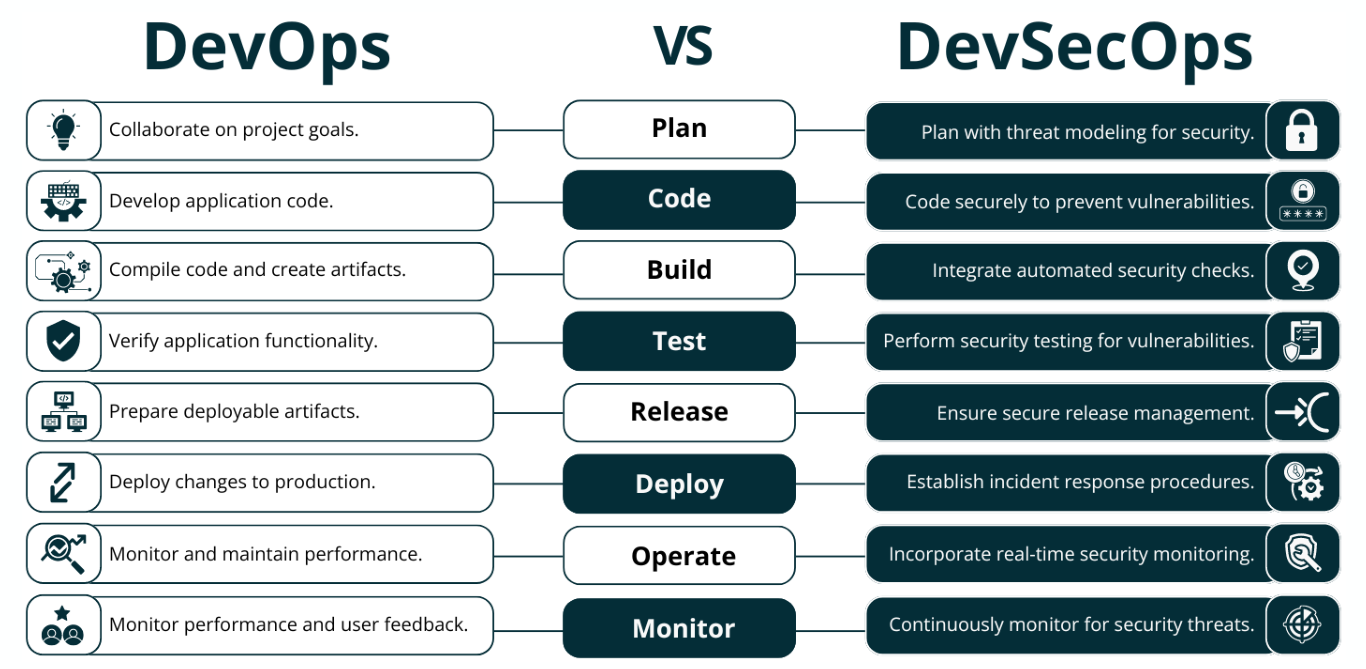
\includegraphics[width=\textwidth]{images/tradsec_vs_devsecops.png}
    \caption{DevOps vs DevSecOps}
\end{figure}

Benefits of DevSecOps include:
\begin{itemize}
    \item   Reduced time to fix bugs: fixing vulnerabilities earlier in development is faster \& cheaper.
    \item   Continuous Security: automated tests \& monitoring ensure security across the pipeline.
    \item   Better Compliance: ensures adherence to industry standards (e.g., GDPR, PCI-DSS) through continuous security checks.
    \item   Improved Collaboration: security becomes a shared responsibility, promoting teamwork.
\end{itemize}

\begin{figure}[H]
    \centering
    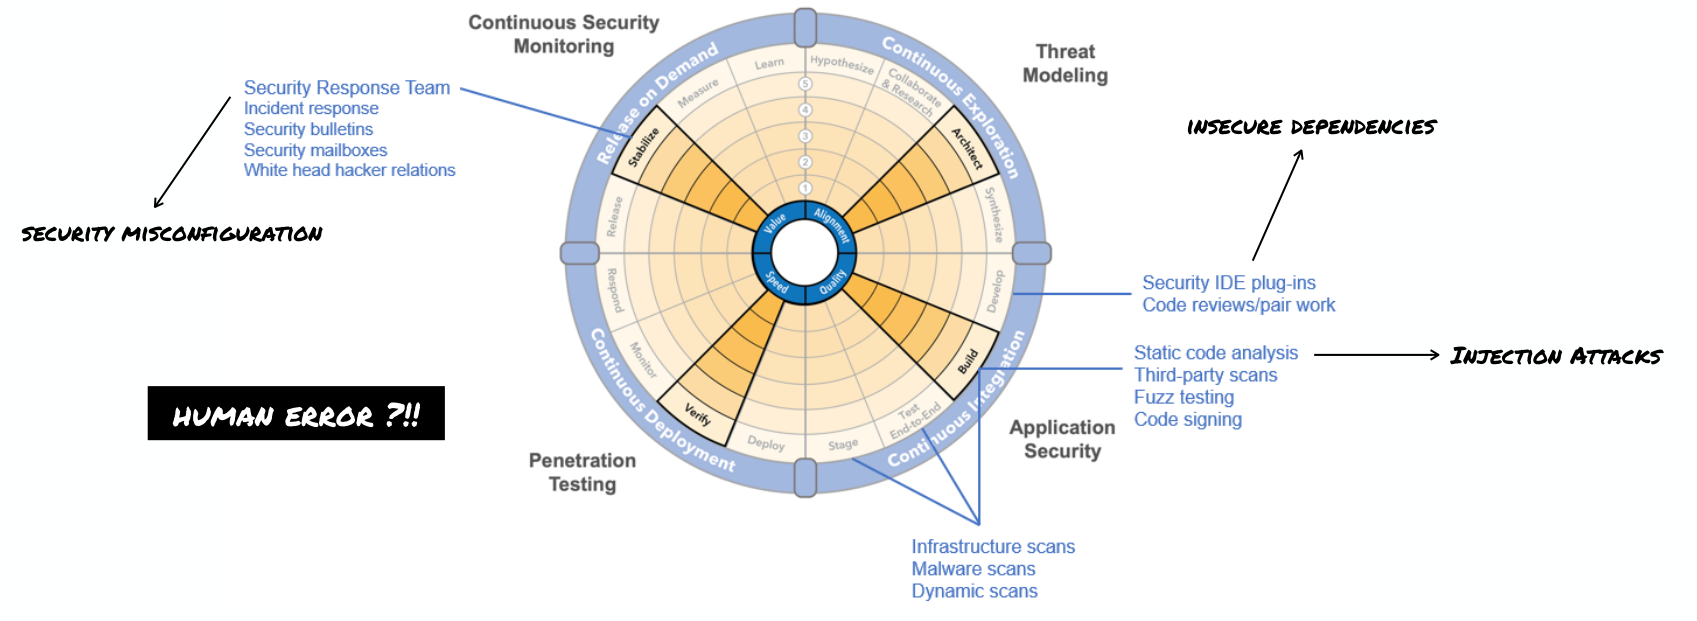
\includegraphics[width=\textwidth]{images/devsecopskeyvulns.png}
    \caption{Key Vulnerabilities}
\end{figure}

Key security metrics include:
\begin{itemize}
    \item   \textbf{Mean Time To Detection:} how fast can you detect security vulnerabilities?
    \item   \textbf{Mean Time To Remediation:} how quickly can you fix vulnerabilities once detected?
    \item   \textbf{Mean Time To Failure:} average amount of time a non-repairable system is expected to function before it fails.
            $$
            \text{MTTF} = \frac{\text{Total Operational Time}}{\text{Number of Failures}}
            $$
    \item   \textbf{Mean Time Before Failures:} similar metric to MTTF but for repairable systems that includes the time to failure and the time it takes to repair the system.
            $$
            \text{Mean Time Between failures} = \text{Mean Time To Detection} + \text{Mean Time To Remediation}
            $$
\end{itemize}

DevSecOps best practices include:
\begin{itemize}
    \item   \textbf{Security as Code:} treat security policies \& tests like code.
            Use version control, collaboration, \& automation reduces attack vectors from the start of the development process.
    \item   \textbf{Automated Testing:} integrate automated security testing into CI/CD pipelines (static, dynamic, \& dependency checks).

    \item   \textbf{Continuous Monitoring:} implement tools for real-time monitoring of security events in production.

    \item   \textbf{Infrastructure as Code (IaC):} automate secure configurations of infrastructure to avoid security misconfigurations.

    \item   \textbf{Training \& Awareness:} regularly train teams on the latest security practices \& vulnerabilities.
\end{itemize}

\subsection{Security Vulnerabilities in Code}
\textbf{Security vulnerabilities} are weaknesses in a system or application that attackers can exploit to compromise confidentiality, integrity, or availability.
Understanding common vulnerabilities is key in building more secure applications, particularly in a DevSecOps pipeline.
Common vulnerabilities include:
\begin{itemize}
    \item   SQL injection.
    \item   Cross-Site Scripting (XSS).
    \item   Cross-Site Request Forgery (CSRF).
    \item   Insecure deserialisation.
    \item   Impoper input validation.
\end{itemize}

\subsubsection{SQL Injection}
\textbf{SQL injection} is a technique wherein attackers manipulate an application's SQL queries by injecting malicious SQL code through user inputs (e.g., forms or URL parameters).
If user input is not properly sanitised, the attacker can execute arbitrary queries to retrieve, modify, or delete sensitive data.
Types of SQL injection include:
\begin{itemize}
    \item   \textbf{Classic SQL injection:} occurs by inserting SQL queries in user inputs.
    \item   \textbf{Blind SQL injection:} SQL queries are injected without knowing the output.
    \item   \textbf{Error-Based SQL injection:} an attacker retrieves information from error messages returned by the database.
\end{itemize}

SQL injection can be prevented with:
\begin{itemize}
    \item   \textbf{Input validation:} ensure all user inputs are properly validated.
    \item   \textbf{Parameterised queries:} use placeholders for query parameters to prevent direct user input into SQL queries.
    \item   \textbf{Stored procedures:} use database-stored procedures instead of dynamic SQL queries.
    \item   \textbf{ORM Frameworks:} use Object-Relational Mapping tools such as JPA which generate secure queries.
    \item   \textbf{Least privilege:} ensure that the database user has minimal privileges.
\end{itemize}

\subsubsection{Cross-Site Scripting}
\textbf{Cross-Site Scripting (XSS)} is a type of injection attack wherein malicious scripts are injected into otherwise benign \& trusted websites.
The attacker tricks the victim's browser into executing malicious scripts, potentially compromising sensitive information such as cookies or login tokens.
Types of XSS include:
\begin{itemize}
    \item   \textbf{Stored XSS:} a malicious script is permanently stored on a target server, e.g. in a database.
            When users visit the page, the malicious script is delivered to their browser from the server.
    \item   \textbf{Reflected XSS:} the injected script is reflected off a web server, often via an error message or search result.
        The user is tricked into clicking a malicious link, where the script is injected and executed.
    \item   \textbf{DOM-based XSS:} the vulnerability occurs in the browser rather than the server.
            The malicious script is part of the Document Object Model.
\end{itemize}

Dangers of XSS include:
\begin{itemize}
    \item   \textbf{Data theft:} attackers can steal cookies, local storage data, \& other sensitive information.
    \item   \textbf{Session hijacking:} attackers can impersonate users by stealing session tokens.
\end{itemize}

XSS can be mitigated with:
\begin{itemize}
    \item   \textbf{Input validation:} always validate \& sanitise user inputs.
    \item   \textbf{Escaping user output:} escape any user input before rendering it in the HTML.
    \item   \textbf{Content Security Policy (CSP):} use a strict CSP to block inline scripts, and only allow trusted scripts to be executed.
    \item   \textbf{HTTPOnly Cookies:} prevent JavaScript from accessing cookies.
\end{itemize}

\subsubsection{Cross-Site Request Forgery}
\textbf{Cross-Site Request Forgery (CSRF)} is an attack wherein a user is tricked into performing actions they didn't intend to by sending an unauthorised request to a trusted web application.
This usually happens when the user is already authenticated and their browser automatically includes credentials (e.g., cookies, tokens).
For example, a malicious website could contain a form that sends a request to a bank's API to transfer money; if the user is already logged into their bank account and visit this webpage, the browser will send the request with the user's bank credentials without them knowing.

\subsection{Static Code Analysis}
\textbf{Static code analysis} is the process of analysing source code without executing it to find potential errors, vulnerabilities, \& coding violations.
It helps to identify weaknesses early in the development process, preventing security vulnerabilities, bugs, \& performance issues before they reach production.
Key metrics include:
\begin{itemize}
    \item   \textbf{Code Complexity:} how difficult is it to understand, test, \& maintain a codebase.
            It's often measured using \textbf{cyclomatic complexity} which counts the number of independent paths through a program's source code by counting the number of decision points (e.g., \mintinline{javascript}{if}, \mintinline{javascript}{while}, \& \mintinline{javascript}{for} statements in the code.
            The higher the complexity, the more testing \& resources are required to ensure stability.
            \\\\
            High complexity indicates that a piece of code has many decision points, which can increase the likelihood of bugs, make it harder to test, \& make the code more prone to errors.
            Low complexity is often associated with cleaner, more maintainable code.
            \\\\
            It is considered best practice to refactor large functions into smaller, more manageable functions and to keep functions \& classes single-responsibilty.


    \item   \textbf{Code Duplication:} this occurs when the same block of code appears multiple times in a codebase.
            This leads to redundancy, increased maintenance costs, \& the potential for inconsistency.
            It is a code smell that increases the risk of errors during future modifications, as if a bug is found in one piece of duplicated code, all other copies of that code need to be fixed as well.
            It leads to code that is harder to refactor, test, \& maintain.
            \\\\
            Best practice to avoid code duplication includes following the DRY (Don't Repeat Yourself) principle, refactoring  duplicated code into reusable functions, and to use inheritance or composition to remove repeated logic between classes.


    \item   \textbf{Code Smells:} these are symptoms in the source code that \textit{might} be indicative of deeper problems.
            They aren't necessarily bugs, but they make code harder to maintain and evolve over time.
            They often point to violations of coding principles or patterns that might lead to future issues.
            Examples include:
            \begin{itemize}
                \item   \textbf{Long methods:} methods that do too much, making them harder to read, test, \& maintain.
                \item   \textbf{Large classes:} classes that handle too many responsibilities, making them complex.
                \item   \textbf{Primitive obsession:} overuse of basic data types instead of creating more meaningful classes.
                \item   \textbf{Feature envy:} a method in one class that heavily relies on the internal data of another class.
                \item   \textbf{God object:} a class that knows too much or does too much, violating the Single Responsibility principle.
            \end{itemize}

            Code smells indicate areas that need refactoring.
            While they may not be immediate bugs, they make the code harder to manage in the long run are are often signs of technical debt.
            Best practice includes refactoring large classes \& methods into smaller, focused components, applying design patterns like Strategy, Factory, or Observer to fix specific code smells, and following SOLID (Single Responsibility, Open-Closed, etc.) principles to avoid common smells.
\end{itemize}

Static code analysis works by performing:
\begin{enumerate}
    \item   \textbf{Scanning:} automated tools analyse source code for predefined patterns \& rules.
    \item   \textbf{Analysis:} tools break down the code and check for common vulnerabilities.
    \item   \textbf{Reporting:} the analysis generates reports categorising findings as bugs, code smells, vulnerabilities, or performance issues.
\end{enumerate}

Key benefits of static code analysis include:
\begin{itemize}
    \item   \textbf{Early bug detection:} reduces future costs by catching bugs early.
    \item   \textbf{Improved code quality:} ensures adherence to coding standards \& best practices.
    \item   \textbf{Security improvements:} identifies security vulnerabilities.
    \item   \textbf{Efficiency:} automated \& continuous scanning of large codebases.
    \item   \textbf{CI/CD integration:} seamless integration with DevOps pipelines.
\end{itemize}

Types of static code analysis include:
\begin{itemize}
    \item   \textbf{Lexical analysis:} analyses tokens \& basic structures like variables \& operators.
    \item   \textbf{Syntax analysis:} examines the structure of the code \& syntax rules.
    \item   \textbf{Semantic analysis:} ensures that the logic of the code makes sense.
    \item   \textbf{Data flow analysis:} examines how data flows through the program to identify unused variables or null pointer exceptions.
\end{itemize}

Tools for static code analysis include:
\begin{itemize}
    \item   \textbf{SonarQube:} supports Java, JavaScript, Python, etc. and features bug detection, vulnerability detection, code smells, \& technical debt.
    \item   \textbf{ESLint:} supports JavaScript and features style guide enforcement \& best practices.
    \item   \textbf{Checkmarx:} focuses on security and features vulnerability detection \& OWASP Top 10 compliance.
    \item   \textbf{FindBugs:} supports Java and features detection of bug patterns in Java bytecode.
\end{itemize}

Best practices for static code analysis include:
\begin{itemize}
    \item   \textbf{Integrate early:} apply static analysis from the beginning of the development cycle.
    \item   \textbf{Automate in CI/CD Pipelines:} ensure continuous scanning for every commit or build.
    \item   \textbf{Review findings regularly:} don't ignore reports, address issues promptly.
    \item   \textbf{Tune rules:} customise analysis rules based on the project requirements.
    \item   \textbf{Complement with manual code reviews:} tools can't detect everything, manual reviews are still necessary.
\end{itemize}

Limitations of static code analysis include:
\begin{itemize}
    \item   \textbf{False positives:} not all flagged issues are real problems, requiring manual inspection.
    \item   \textbf{No runtime error detection:} unlike dynamic analysis, it can't identify errors that only occur during execution.
    \item   \textbf{Context ignorance:} might not understand the broader context of the code.
    \item   \textbf{Performance overhead:} large codebases can take time to analyse thoroughly.
\end{itemize}

\section{Software Security}
\textbf{Software security} is the concept of implementing mechanisms \& adopting best development practices to protect software against malicious attacks, i.e. to make it resistant to attacks and to keep it functional when attacked.
In traditional software design \& development practices, software security was almost an afterthought.
Secure software is defined as software engineered in such a way that its operation and functionality continues as normal even when subjected to malicious attacks.
\\\\
In computer security, a \textbf{threat} is a potential negative action or event facilitated by a vulnerability that results in an unwanted impact to a computer system or application.
A threat can either be a negative \textit{intentional} event such as a cyberattack, or an \textit{accidental} even such as an earthquake.
Different definitions from different authorities for what constitutes a threat include:
\begin{itemize}
    \item   \textbf{ISO27005:} a potentital cause of an incident that may result in harm of systems \& organisation.
    \item   \textbf{NIST:} any circumstance or event with the potential to adversely impact organisation operations, organisational assets, or individuals through an information system via unauthorised access, destruction, disclosure, modification of information, and / or denial of service.
    \item   \textbf{ENISA:} any circumstance or event with the potential to adversely impact an asset through unauthorised access, destruction, disclosure, modification of data, and / or denial of service.
\end{itemize}

\subsection{Threat Classification}
Microsoft classifies threats into the following categories:
\begin{itemize}
    \item   \textbf{Spoofing of user identity:} e.g., an attacker takes on the identity of an administrator.
    \item   \textbf{Tampering:} e.g., an attacker changes an account balance.
    \item   \textbf{Repudiation:} e.g., a user denies performing an action without either parties having any way to prove otherwise.
    \item   \textbf{Information disclosure:} privacy breach or data leak.
    \item   \textbf{Elevation of privilege:} an attacker elevates their own security level to an administrator.
    \item   \textbf{Denial of Service (DOS):} a cyber attack in which the perpetrator seeks to make a machine or network resource unavailable to its intended users by temporarily or indefinitely disrupting services of a host connected to the internet.
\end{itemize}

The term \textbf{threat agent} is used to indicate an individual, thing, or a group that can manifest a threat.
These incldue:
\begin{itemize}
    \item   Non-target specific, e.g. a computer virus, worms, trojans, \& logic bombs.
    \item   Employees, e.g. disgruntled staff or contractors.
    \item   Organised crime \& criminals.
    \item   Corporation, e.g. partners or competitors.
    \item   Human (unintentional), e.g., accidents, carelessness.
    \item   Human (intentional), insider, outsider.
    \item   Natural, e.g., flood, fire, lighting, meteor, earthquakes.
\end{itemize}

\subsubsection{Requirement-Level Threats}
Expertise in requirements engineering \& information system security is a rare combination: customers \& users don't know what they want with respect to security, and requirement engineers don't know what questions to ask to elicit security requirements.
This combined lack of security expertise leads to missing or unidentified security requirements, resulting in security vulnerabilities.

\subsubsection{Hardware-Level Threats}
\begin{table}[h!]
    \centering

    \begin{tabular}{|>{\arraybackslash}p{0.5\textwidth}|>{\arraybackslash}p{0.5\textwidth}|}
        \hline
        \textbf{Threat}                             & \textbf{Countermeasure} \\ \hline
        Eavesdropping devices (e.g., keyloggers)    & Physical Security \\ \hline
        Power outage                                & Uninterruptible Power Supply \\ \hline
        Natural Disasters                           & Geographically dispersed redundancy to avoid a single point of failure \\ \hline
        Sabotage & Physical Security \\ \hline
    \end{tabular}
    \caption{Hardware-Level Threats \& Countermeasures}
\end{table}

\subsubsection{Code-Level Threats}
Code-level threats include \textbf{unintentional} threats, which are mainly caused by a lack of secure coding knowledge.
These can be mitigated with software security education \& training, automatic static \& dynamic code analysis, and peer code review.
\\\\
\textbf{Intentional} threats can be prevented with peer code review, job rotation, \& mandatory vacation.

\subsubsection{Design-Level Threats}
\textbf{Design-level threats} relate to weaknesses in principal OO design \& object interaction, therefore secure design is more fundamental than secure coding, e.g., object attributes being public rather than private.
Best OO design practices are captures in design patterns for security.
Code implementation without a solid design is dangerous \& costly.

\subsubsection{Architectural-Level Design Threats}
\textbf{Architectural design} decisions entail overarching design decisions.
Widely accepted solutions to these recurring architectural design problems are referred to as \textbf{architectural patterns}.


\end{document}
